\documentclass[10pt]{article}

% Packages and macros go here
\usepackage[T1]{fontenc}
\usepackage{lmodern}
\usepackage[utf8x]{inputenx}
\usepackage{microtype}
\usepackage{framed}
\usepackage{listings}
\usepackage{vmargin}
\usepackage{setspace}
\usepackage{mathrsfs, mathenv}
\usepackage{amsmath, amsthm, amssymb, amsfonts, amscd}
\usepackage{graphicx}
\usepackage{epstopdf}
\usepackage[svgnames]{xcolor}
\usepackage{hyperref}
\usepackage[capitalise]{cleveref}
\hypersetup{citecolor=blue, colorlinks=true, linkcolor=black}
\setlength{\parskip}{6pt}
\setlength\parindent{0pt}
\usepackage{subcaption}
\usepackage{bbm}
\usepackage{cite}
\usepackage{verbatim}
\usepackage{pgfplots}
\usepackage{tikz}
\usepackage{etoolbox}
\usepackage{color}
\usepackage{lipsum}
\usepackage{ifthen}
\usepackage[linesnumbered, ruled, vlined]{algorithm2e}
\crefname{algocf}{Algorithm}{Algorithms}
\usepackage{autonum}

\theoremstyle{plain}
\newtheorem{theorem}{Theorem}[section]
\newtheorem{corollary}[theorem]{Corollary}
\newtheorem{lemma}[theorem]{Lemma}
\newtheorem{proposition}[theorem]{Proposition}
\numberwithin{equation}{section}

\theoremstyle{definition}
\newtheorem{definition}[theorem]{Definition}

\theoremstyle{remark}
\newtheorem{remark}[theorem]{Remark}
\newtheorem{assumption}[theorem]{Assumption}
\newtheorem{example}[theorem]{Example}


\ifpdf
  \DeclareGraphicsExtensions{.eps,.pdf,.png,.jpg}
\else
  \DeclareGraphicsExtensions{.eps}
\fi

\usepackage{mathtools}
% basics

% tables
\usepackage{booktabs}

% plots
\usepackage{pgfplots}
\usepackage{tikz}
\usetikzlibrary{patterns,arrows,decorations.pathmorphing,backgrounds,positioning,fit,matrix}
\usepackage[labelfont=bf]{caption}
\setlength{\belowcaptionskip}{-5pt}
\usepackage{here}
\usepackage[font=normal]{subcaption}

% Prevent itemized lists from running into the left margin inside theorems and proofs
\usepackage{enumitem}
\setlist[itemize]{leftmargin=.5in}
\setlist[enumerate]{leftmargin=.5in,topsep=3pt,itemsep=3pt,label=(\roman*)}

% Add a serial/Oxford comma by default.
\newcommand{\creflastconjunction}{, and~}

% Sets running headers as well as PDF title and authors
% title and authors

\newcommand{\email}[1]{\href{#1}{#1}}
\newcommand{\TheTitle}{Probabilistic methods for elliptic partial differential equations} 
\newcommand{\TheAuthors}{A. Abdulle, G. Garegnani}
%\headers{Random time steps for quantifying chaotic numerical integration}{\TheAuthors}
\title{{\TheTitle}}
\newcommand*\samethanks[1][\value{footnote}]{\footnotemark[#1]}
\author{Assyr Abdulle\thanks{Institute of Mathematics, \'Ecole Polytechnique F\'ed\'erale de Lausanne (\email{\{assyr.abdulle, giacomo.garegnani\}@epfl.ch})}
	\and
	Giacomo Garegnani\samethanks}
\date{}

\usepackage{amsopn}
\DeclareMathOperator{\diag}{diag}
\DeclarePairedDelimiter{\ceil}{\left\lceil}{\right\rceil}
\DeclarePairedDelimiter{\floor}{\lfloor}{\rfloor}
\DeclarePairedDelimiter{\abs}{\lvert}{\rvert}
\DeclarePairedDelimiter{\norm}{\lVert}{\rVert}
\renewcommand{\phi}{\varphi}
\renewcommand{\theta}{\vartheta}
\renewcommand{\Pr}{\mathbb{P}}
\newcommand{\btilde}{\widetilde}
\newcommand{\bhat}{\widehat}
\newcommand{\eqtext}[1]{\ensuremath{\stackrel{#1}{=}}}
\newcommand{\leqtext}[1]{\ensuremath{\stackrel{#1}{\leq}}}
\newcommand{\iid}{\ensuremath{\stackrel{\text{i.i.d.}}{\sim}}}
\newcommand{\totext}[1]{\ensuremath{\stackrel{#1}{\to}}}
\newcommand{\rightarrowtext}[1]{\ensuremath{\stackrel{#1}{\longrightarrow}}}
\newcommand{\leftrightarrowtext}[1]{\ensuremath{\stackrel{#1}{\longleftrightarrow}}}
\newcommand{\pdv}[2]{\ensuremath\partial_{#2}#1}
\newcommand{\N}{\mathbb{N}}
\newcommand{\R}{\mathbb{R}}
\newcommand{\C}{\mathbb{C}}
\newcommand{\OO}{\mathcal{O}}
\newcommand{\epl}{\varepsilon}
\newcommand{\diffL}{\mathcal{L}}
\newcommand{\prior}{\mathcal{Q}}
\newcommand{\defeq}{\coloneqq}
\newcommand{\eqdef}{\eqqcolon}
\newcommand{\Var}{\operatorname{Var}}
\newcommand{\E}{\operatorname{\mathbb{E}}}
\newcommand{\MSE}{\operatorname{MSE}}
\newcommand{\trace}{\operatorname{tr}}
\newcommand{\MH}{\mathrm{MH}}
\newcommand{\ttt}{\texttt}
\newcommand{\Hell}{d_{\mathrm{H}}}
\newcommand{\sksum}{{\textstyle\sum}}
\newcommand{\dd}{\, \mathrm{d}}
\renewcommand{\d}{\mathrm{d}}
\definecolor{shade}{RGB}{100, 100, 100}
\definecolor{bordeaux}{RGB}{128, 0, 50}
\newcommand{\corr}[1]{{\color{red}#1}}
\newcommand{\Tau}{\tau}
\newcommand{\LL}{L}
\newcommand{\HH}{H}
\newcommand{\WW}{W}
\newcommand{\mbf}{\mathbf}
\newcommand{\bfs}{\boldsymbol}
\newcommand{\todo}{{\color{red} TO DO}}
\newcommand{\X}{\mathbb{X}}
\newcommand{\nablar}{\nabla_{\hat x}}
\newcommand{\eval}[1]{\bigr\rvert_{#1}}
\newcommand{\normm}[1]{\norm{#1}_a}
%\newcommand{\normm}[1]{{\left\vert\kern-0.25ex\left\vert\kern-0.25ex\left\vert #1 
%		\right\vert\kern-0.25ex\right\vert\kern-0.25ex\right\vert}}

\usepackage[usestackEOL]{stackengine}
\newcommand\fop[3][9pt]{\mathop{\ensurestackMath{\stackengine{#1}%
			{\displaystyle#2}{\scriptstyle#3}{U}{c}{F}{F}{L}}}\limits}
\newcommand\finf[2][9pt]{\fop[#1]{\inf}{#2}}
\newcommand\fsum[2][14pt]{\fop[#1]{\sum}{#2}}

\definecolor{leg1}{RGB}{0,114,189}
\definecolor{leg2}{RGB}{217,83,25}
\definecolor{leg3}{RGB}{237,177,32}
\definecolor{leg4}{RGB}{126,47,142}
\definecolor{leg5}{RGB}{119,172,48}

\definecolor{leg21}{RGB}{62,38,169}
\definecolor{leg22}{RGB}{46,135,247}
\definecolor{leg23}{RGB}{55,200,151}
\definecolor{leg24}{RGB}{254,195,56}


\ifpdf
\hypersetup{
	pdftitle={\TheTitle},
	pdfauthor={\TheAuthors}
}
\fi


\begin{document}
\maketitle	

\begin{abstract} The abstract goes here.
\end{abstract}	

\textbf{AMS subject classifications.} 62G05, 65N21, 74Q05.

\textbf{Key words.} Inverse problems, Multiscale modelling, Homogenization, Ensemble Kalman filter, Bayesian inference, Modelling error.

\section{Introduction}

\section{Problem setting}

Let us consider multiscale inverse problems of the following form
\begin{equation}
\label{multiscale_inverse_problem}
\text{find } u^{\varepsilon} \in X \text{ given observations } y = \mathcal{G}^{\varepsilon}(u^{\varepsilon}) + \eta \in Y,
\end{equation}
where the parameter space $X$ and the observation space $Y$ are Hilbert spaces, $\mathcal{G}^{\varepsilon} \colon X \to Y$ is the forward response operator mapping the unknown $u$ to the observation space, and $\eta \in Y$ is a source of additive noise, modelled as a mean zero random variable with covariance operator $\Gamma$. Usually, in applications, the forward operator $\mathcal{G}^{\varepsilon}$ can be written as $\mathcal{G}^{\varepsilon} = \mathcal{O} \circ \mathcal{S}^{\varepsilon}$, where $\mathcal{O} \colon H^1_0(\Omega) \to Y$ is an observation operator and $\mathcal{S}^{\varepsilon}$ is the solution operator of a multiscale partial differential equation (PDE). Let $\Omega$ be a bounded open domain, $\mathcal{S}^{\varepsilon}$ maps the unknown $u$ to the solution $p^{\varepsilon}$ of 
\begin{equation}
\label{intro_problem_multiscale}
\begin{cases}
- \nabla \cdot ( A^{\varepsilon}_u \nabla p^{\varepsilon} ) = 0 & \text{ in } \Omega, \\
p^{\varepsilon} = 0 & \text{ on } \partial \Omega,
\end{cases}
\end{equation}
therefore $\mathcal{S}^{\varepsilon} \colon X \to H^1_0(\Omega)$ and $\mathcal{O} \colon H^1_0(\Omega) \to Y$, for which we assume that the following property holds true.
\begin{assumption}
\label{ass_O}
\leavevmode \\
The observation operator $\mathcal{O} \colon H^1_0(\Omega) \to Y$ satisfies for all $p_1, p_2 \in H^1_0(\Omega)$
\[ \norm{\mathcal{O}(p_1) - \mathcal{O}(p_2)}_2 \le m \norm{p_1 - p_2}_{L^2(\Omega)}, \]
where $m$ is a positive constant.
\end{assumption}
Note that Assumption \ref{ass_O} is a stronger property than being Lipschitz.
The tensor $A^{\varepsilon}_u$ belongs to the class of parametrized multiscale tensors which admit explicit scale separation between slow and fast spatial variables
\begin{equation*}
A^{\varepsilon}_u(x) = A \left ( u(x), \frac{x}{\varepsilon} \right ),
\end{equation*}
where the map $(t,x) \to A \left ( t, \frac{x}{\varepsilon} \right )$ is assumed to be known and $A$ is periodic in its second argument. \\
If $\varepsilon$ is small, we have to employ a fine discretization to resolve the smallest scale in the evaluation of $\mathcal{G}^{\varepsilon}$, which in turn leads to a high computational cost. Considering also that the PDE has to be solved several times in the framework of inverse problems, this procedure can be infeasible. \\
Therefore, we apply the homogenization theory (see e.g. \cite{CiD99}), which ensures the existence of an homogenized tensor $A^0$, such that the solution $p^0$ of the problem 
\begin{equation}
\label{intro_problem_homogenized}
\begin{cases}
- \nabla \cdot ( A^0_u \nabla p^0 ) = 0 & \text{ in } \Omega, \\
p^0 = 0 & \text{ on } \partial \Omega,
\end{cases}
\end{equation}
is the weak limit for $\varepsilon \to 0$ of the functions $p^{\varepsilon}$, i.e.
\begin{equation*}
p^{\varepsilon} \rightharpoonup p^0 \qquad \text{in } H^1(\Omega).
\end{equation*}
Hence, the function $p^0$ is a good approximation of $p^{\varepsilon}$ when the multiscale parameter $\varepsilon$ is
small and, in this case, the multiscale problem \eqref{intro_problem_multiscale} can be replaced by its homogenized version \eqref{intro_problem_homogenized}. In order to solve numerically \eqref{intro_problem_homogenized}, we adopt a finite element discretization and we denote $\mathcal{G}^0_h \colon \mathcal{O} \circ \mathcal{S}^0_h$ the forward operator which involves the solution of this problem. Thus, even if, as written in \eqref{multiscale_inverse_problem}, the observations of the inverse problem come from a multiscale model represented by the forward operator $\mathcal{G}^{\varepsilon}$, inspired by \cite{NPS12}, we employ the forward operator given by its discrete homogenized version $\mathcal{G}^0_h$ to solve the inverse problem. Finally, we introduce assumptions on the multiscale and homogenzed tensors $A^{\varepsilon}$ and $A^0$.
\begin{assumption}
\label{ass_A}
\leavevmode \\
The tensors $A^{\varepsilon}$ for the multiscale problem \eqref{intro_problem_multiscale} and $A^0$ for the homogenized problem \eqref{intro_problem_homogenized} satisfy for all $u, u_1, u_2 \in X$
\begin{align*}
& \norm{A^{\varepsilon}(u_1) - A^{\varepsilon}(u_2)}_{L^{\infty}(\Omega;\R^{N \times N})} \le M \norm{u_1 - u_2}_X, \\
& \norm{A^0(u_1) - A^0(u_2)}_{L^{\infty}(\Omega;\R^{N \times N})} \le M \norm{u_1 - u_2}_X,
\end{align*}
and
\begin{equation*}
A^{\varepsilon}(u) \xi \cdot \xi \ge \alpha_0 \norm{\xi}_2^2, \quad A^0(u) \xi \cdot \xi \ge \alpha_0 \norm{\xi}_2^2, \qquad \text{for all } \xi \in \R^N,
\end{equation*}
where $M$ and $\alpha_0$ are positive constants.
\end{assumption}

\section{Ensemble Kalman filter for multiscale inverse problems}

We solve the inverse problem by applying the ensemble Kalman filter $\mathrm{EnKF}$, for which we present here a small introduction and refer to \cite{ILS13} for further details. Differently from our work, in \cite{ILS13} the authors apply the ensemble Kalman method to one-scale inverse problems. \\
Inverse problems are often ill-posed and they require regularization, which can be achieved through many techniques, both variational and Bayesian. In this method regularization is
obtained by searching for the solution in a finite dimensional and compact subset $\mathcal{A}$ of $X$, which incorporates prior knowledge of $u$. In order to approximate the true unknown by means of the Kalman filter theory, we need to introduce artificial dynamics based on state augmentation. \\
We define the space $Z = X \times Y$ and the mapping $\Xi \colon Z \to Z$ by 
\[ \Xi(z) = \begin{bmatrix} u \\ \mathcal{G}^0_h(u) \end{bmatrix}, \quad \text{ for } \quad z = \begin{bmatrix} u \\ v \end{bmatrix} \in Z, \]
which induces artificial dynamics as
\[ z_{n+1} = \Xi(z_n). \]
We assume that data related to the artificial dynamics has the form
\[ y_{n+1} = H z_{n+1} + \eta_{n+1}, \]
where $H \colon Z \to Y$ is a projection operator defined by $H = \begin{bmatrix} 0 & I \end{bmatrix}$ and
$\{ \eta_n \}_{n \in \mathbb{N}}$ is an i.i.d. sequence of random variables distributed as $\eta_n \sim \mathcal{N}(0,\Gamma)$.
Consequently we get 
\[ y_{n+1} = H \Xi(z_n) + \eta_{n+1} = \mathcal{G}^0_h(u_n) + \eta_{n+1}. \]
The ensemble Kalman method uses an ensemble of states of dimension $J$, which is sequentially updated by means of the Kalman formula for $N$ iterations. The last detail missing  is the initial ensemble of particles $\{ z_0^{(j)} \}_{j = 1}^J$. This first guess can be defined by constructing an ensemble $\{ \psi^{(j)} \}_{j = 1}^J$ in $X$ and taking 
\begin{equation*}
z_0^{(j)} = \begin{bmatrix} \psi^{(j)} \\ \mathcal{G}^0_h(\psi^{(j)}) \end{bmatrix}.
\end{equation*}
The initial ensemble is related to the definition of the space $\mathcal{A}$, which incorporates prior knowledge of the solution. We assume that the prior knowledge is a probability measure denoted by $\mu_0$, then $\{ \psi^{(j)} \}_{j = 1}^J$ is constructed drawing $J$ samples from this distribution. Finally, the set $\mathcal{A}$ is given by the subspace generated by the initial ensemble members
\[ \mathcal{A} = \mathrm{span} \; \{\psi^{(j)} \}_{j=1}^J. \]
Each iteration of the ensemble Kalman method is divided in two steps: prediction and analysis. In the first step we map the current ensemble of particles $\{ z_n^{(j)} \}_{j=1}^J$ into the data space, introducing information about the forward model $\mathcal{G}^0_h$, which is contained in the definition of $\Xi$, and obtaining prior estimates of the state variables
\begin{equation*}
\hat{z}_{n+1}^{(j)} = \Xi(z_n^{(j)}).
\end{equation*}
In the second step the ensemble of particles $\{ z_n^{(j)} \}_{j=1}^J$ is updated comparing the mapped ensemble $\{ H \hat{z}_{n+1}^{(j)} \}_{j=1}^J$ with versions of the data perturbed with noise $\{ y_{n+1}^{(j)} \}_{j=1}^J$ via the standard Kalman update formula
\begin{equation}
z_{n+1}^{(j)} = \hat{z}_{n+1}^{(j)} + K_{n+1} (y_{n+1}^{(j)} - H \hat{z}_{n+1}^{(j)}) = (I - K_{n+1} H) \hat{z}_{n+1}^{(j)} + K_{n+1} y_{n+1}^{(j)},
\end{equation}
where $y_{n+1}^{(j)} = y + \eta_{n+1}^{(j)}$ and
\begin{equation*}
K_{n+1} = C_{n+1} H^* (H C_{n+1} H^* + \Gamma)^{-1},
\end{equation*}
where $H^*$ is the adjoint operator of $H$ and
\begin{equation*}
C_{n+1} = \frac{1}{J} \sum_{j = 1}^J (\hat{z}_{n+1}^{(j)} - \bar{z}_{n+1}) (\hat{z}_{n+1}^{(j)} - \bar{z}_{n+1})^T = \frac{1}{J} \sum_{j = 1}^J \hat{z}_{n+1}^{(j)} (\hat{z}_{n+1}^{(j)})^T - \bar{z}_{n+1} \bar{z}_{n+1}^T.
\end{equation*}
Note that the update equation for the unknown is
\begin{equation*}
u_{n+1}^{(j)} = u_n^{(j)} + C_{n+1}^{up} ( C_{n+1}^{pp} + \Gamma )^{-1} (y_{n+1}^{(j)} - \mathcal{G}(u_n^{(j)})). 
\end{equation*}
Finally, the solution is computed by averaging over the ensemble of particles
\begin{equation*}
u_{\mathrm{EnKF}} = \frac{1}{J} \sum_{j = 1}^J H^{\perp} z_{N}^{(j)} = \frac{1}{J} \sum_{j = 1}^J u_{N}^{(j)},
\end{equation*}
where $H^{\perp} \colon Z \to Y$ is a projection operator defined by $H^{\perp} = \begin{bmatrix} I & 0 \end{bmatrix}$.

\begin{remark}
\leavevmode \\
The computational cost of the iterative ensemble Kalman algorithm can be measured in terms of the number of evaluations of the forward operator, indeed the operations to compute the Kalman gain and update the ensemble of particles are negligible with respect to the resolution of the homogenized problem, which is the most expensive task. Therefore, the complexity of the algorithm is $\mathcal{O}(JN)$, where $J$ is the dimension of the ensemble and $N$ is the number of iterations. Moreover, note that the ensemble Kalman method is easily parallelizable. Indeed, at each iteration, we apply the forward operator to every particle in the ensemble individually. Hence, if we call $n_{\mathrm{CPU}}$ the number of central processing units available and we neglect the cost of exchanging of information between processors, the computational cost of the iterative ensemble Kalman method becomes
\[ \mathcal{O} \left ( \frac{J}{n_{\mathrm{CPU}}} N \right ). \]
Thus, if we have a big number of CPUs available, a parallelized version of the code reduces significantly the computational time for the resolution of the inverse problem.
\end{remark}

Following \cite{ScS17}, the ensemble Kalman filter can be interpreted also from a Bayesian point of view. Given a prior distribution $\mu_0$ for the unknown, we want to estimate the conditional posterior distribution $\mu$ of the unknown given the data, which is distributed according to the measure
\begin{equation*}
\mu(du) = \frac{1}{Z} e^{- \Phi(u;y)} \mu_0(du),
\end{equation*}
where $Z$ is a normalization constant and $\Phi(u;y)$ is the least squares functional
\[ \Phi(u;y) = \frac{1}{2} \norm{ \Gamma^{-1/2} (y - \mathcal{G}(u)) }_2^2. \]
We follow an iterative procedure of $N$ steps and we define the intermediate measures
\begin{equation*}
\mu_n(du) = \frac{1}{Z_n} e^{- n \Delta \Phi(u;y)} \mu_0(du),
\end{equation*}
where $\Delta = 1/N$. Note that $\mu_N = \mu$ is the desired final measure. Then we obtain
\begin{equation*}
\mu_{n+1}(du) = \frac{Z_n}{Z_{n+1}} e^{- h \Phi(u;y)} \mu_n(du).
\end{equation*}
The posterior distribution $\mu_n$ is approximated by a sum of Dirac masses centered in the particles of the ensemble at the $n$-th iteration
\begin{equation}
\label{mu_delta}
\mu_n \simeq \frac{1}{J} \sum_{j=1}^J \delta_{u_{n}^{(j)}}.
\end{equation}
The mapping of particles at time $n$ into those at time $n+1$ is given by the ensemble Kalman filter update formula, where $\Gamma$ has been replaced by $\Delta^{-1} \Gamma$
\begin{equation*}
u_{n+1}^{(j)} = u_n^{(j)} + C^{up}(u_n) ( C^{pp}(u_n) + \Delta^{-1} \Gamma )^{-1} (y_{n+1}^{(j)} - \mathcal{G}(u_n^{(j)})).
\end{equation*}
Finally, let us introduce an assumption on the algorithm, which will be employed in the analysis.
\begin{assumption}
\label{ass_algo}
\leavevmode \\
The algorithm is stable, in the sense that all the particles in the ensemble at each iteration lie in the ball $B_R(u^*)$ for some $R > 0$ sufficiently big, where $u^*$ is the true unknown.
\end{assumption}

\section{Convergence analysis}

In this section we show the convergence of the ensemble of particles generated by the $\mathrm{EnKF}$ algorithm using the FEM discretization of the homogenized problem as forward operator to the ensemble of particles generated by the $\mathrm{EnKF}$ algorithm using the multiscale problem as forward operator. Moreover, from the Bayesian perspective, we show the convergence of their posterior distributions. Under further assumptions, we also provide a rate of convergence. The whole analysis is done in the finite dimensional case, where the ensemble of particles lie in $\R^M$ and the observations are in $\R^L$, but it can be generalized to the infinite dimensional setting. Therefore, the forward operators under consideration are $\mathcal{G}^{\varepsilon} \colon \R^M \to \R^L$, $\mathcal{G}^{\varepsilon} = \mathcal{O} \circ \mathcal{S}^{\varepsilon}$ and $\mathcal{G}^0_h \colon \R^M \to \R^L$, $\mathcal{G}^0_h = \mathcal{O} \circ \mathcal{S}^0_h$. We also introduce the forward operator $\mathcal{G}^0 \colon \R^M \to \R^L$, $\mathcal{G}^0 = \mathcal{O} \circ \mathcal{S}^0$, where $\mathcal{S}^0$ is the continuous solution operator of problem \eqref{intro_problem_homogenized}, which maps the unknown $u$ to the solution $p^0$. \\
Given an ensemble of particles $u = \{ u^{(j)} \}_{j = 1}^J$, we define the ensemble norm in the following way
\begin{equation}
\label{ensemble_norm}
\norm{u} \vcentcolon = \frac{1}{J} \sum_{j=1}^J \norm{u^{(j)}}_2,
\end{equation}
and note that it satisfies the properties of a norm
\begin{itemize}
\item $\norm{u} \ge 0$,
\item $\norm{u} = 0$ if and only if $\norm{u^{(j)}}_2 = 0$ for all $j = 1, \dots, J$, which is true if and only if $u^{(j)} = 0$ for all $j = 1, \dots, J$, which is equivalent to $u = 0$,
\item $\norm{\lambda u} = \frac{1}{J} \sum_{j=1}^J \norm{\lambda u^{(j)}}_2 = \abs{\lambda} \frac{1}{J} \sum_{j=1}^J \norm{u^{(j)}}_2 = \abs{\lambda} \norm{u}$,
\item $\norm{u + v} \vcentcolon = \frac{1}{J} \sum_{j=1}^J \norm{u^{(j)} + v^{(j)}}_2 \le \frac{1}{J} \sum_{j=1}^J \left [ \norm{u^{(j)}}_2 + \norm{v^{(j)}}_2 \right ] = \norm{u} + \norm{v}$.
\end{itemize}
In the last point, the sum of two ensembles is intended to be the ensemble whose particles are the sum of the single particles in each ensemble. In the next sections we analyse separately the point-wise convergence of the particles and the convergence of the posterior distributions.

\subsection{Convergence of the point estimate}

The main result is stated in Theorem \ref{convergence_result_full}.
\begin{theorem}
\label{convergence_result_full}
\leavevmode \\
Let $u_{N,h}^0 = \{ u_{N,h}^{0^{(j)}} \}_{j=1}^J$, $u_N^{\varepsilon} = \{ u_N^{\varepsilon^{(j)}} \}_{j=1}^J$ be the ensembles of particles at the last iteration of the iterative ensemble Kalman filter for the forward operators $\mathcal{G}^0_h$ and $\mathcal{G}^{\varepsilon}$ respectively. 
Then, under Assumption \ref{ass_O}, Assumption \ref{ass_A} and Assumption \ref{ass_algo}, we have
\begin{equation*}
\mathbb{E} \left [ \norm{u_N^{\varepsilon} - u_{N,h}^0} \right ] \to 0 \qquad \text{ as } \varepsilon, h \to 0.
\end{equation*}
In particular, if the exact solution $p^0$ of the homogenized problem \eqref{intro_problem_homogenized} is in $H^{q+1}(\Omega)$ with $q \ge 1$, $A^0 \in C^q(\Omega;\R^{N \times N})$, $f \in H^{q-1}(\Omega)$, $\partial \Omega \in C^{q+1}$, and we use polynomials of degree $r$ for the finite element basis, we have the following rate of convergence
\begin{equation*}
\mathbb{E} \left [ \norm{u_N^{\varepsilon} - u_{N,h}^0} \right ] \le C ( \varepsilon + h^{s+1} ),
\end{equation*} 
where $s = \min \{ r, q \}$.
\end{theorem}

We analyse separately the multiscale convergence and the finite element discretization convergence. We first show the convergence of the ensemble of particles generated by the $\mathrm{EnKF}$ algorithm using the multiscale problem as forward operator to the ensemble of particles generated by the $\mathrm{EnKF}$ algorithm using the homogenized problem as forward operator. Then we show the convergence of the ensemble of particles generated by the $\mathrm{EnKF}$ algorithm using a FEM discretization of the homogenized problem as forward operator to the ensemble of particles generated by the $\mathrm{EnKF}$ algorithm using the true homogenized problem as forward operator. \\
Let $e \colon \R \times \R^M \to \R$ be a function modelling the error due to the replacement of the multiscale problem with the homogenized one
\begin{equation}
\label{e}
e(\varepsilon, u) = \frac{1}{J} \sum_{j=1}^J \norm{\mathcal{G}^{\varepsilon}(u^{(j)}) - \mathcal{G}^0(u^{(j)})}_2.
\end{equation}
and $\tilde{e} \colon \R \times \R^M \to \R$ be the error induced by the use of a FEM discretization for the homogenized problem
\begin{equation}
\label{e_tilde}
\tilde{e}(h, u) = \frac{1}{J} \sum_{j=1}^J \norm{\mathcal{G}^0_h(u^{(j)}) - \mathcal{G}^0(u^{(j)})}_2.
\end{equation}
Before proving the main theorem, we need some preliminary results.

\begin{lemma}
\label{lemma_difference_inverse}
\leavevmode \\
Let $A$ and $B$ be square invertible matrices, then
\begin{equation*}
\norm{A^{-1} - B^{-1}}_2 \le \norm{A^{-1}}_2 \norm{B^{-1}}_2 \norm{A - B}_2.
\end{equation*}
\end{lemma}
\begin{proof}
The proof can be found in the appendix.
\end{proof}

\begin{lemma}
\label{lemma_inverse_sum}
\leavevmode \\
Let $A$ and $B$ be square, symmetric matrices, such that $A$ is positive semidefinite and $B$ is positive definite, then
\[ \norm{(A + B)^{-1}}_2 \le \norm{B^{-1}}_2. \]
\end{lemma}
\begin{proof}
The proof can be found in the appendix.
\end{proof}

\begin{lemma}
\label{G_lipschitz}
\leavevmode \\
Let $\mathcal{G} \colon \mathbb{R}^M \to \mathbb{R}^L$, $\mathcal{G} = \mathcal{O} \circ \mathcal{S}$ be the forward operator defined by the composition of an observation operator $\mathcal{O} \colon H^1_0(\Omega) \to \mathbb{R}^L$ and a solution operator $\mathcal{S} \colon \mathbb{R}^M \to H^1_0(\Omega)$, which assigns to $u \in \mathbb{R}^M$ the solution $p \in H^1_0(\Omega)$ of the elliptic partial differential equation
\begin{equation}
\label{problem_lemma}
\begin{cases}
- \nabla \cdot ( {A(u) \nabla p} ) = f & \text{ in } \Omega, \\
p = 0 & \text{ on } \partial \Omega,
\end{cases}
\end{equation}
where $\Omega \subset \R^N$ is a domain, $A(u) \in L^{\infty}(\Omega; \R^{N \times N})$ and $f \in L^2(\Omega)$.
Let $\mathcal{O}$ be Lipschitz and $A$ such that
\[ \norm{A(u_1) - A(u_2)}_{L^{\infty}(\Omega; \R^{N \times N})} \le M \norm{u_1 - u_2}_2, \]
and
\[ A(u) \xi \cdot \xi \ge \alpha \norm{\xi}_2^2 \qquad \text{ for all } \xi \in \mathbb{R}^N, \]
where $M$ and $\alpha$ are positive constants. Then $\mathcal{G}$ is Lipschitz.
\end{lemma}
%\begin{proof}
%The proof can be found in the appendix.
%\end{proof}
\begin{proof}
Let $u_1, u_2 \in \mathbb{R}^M$, then the weak formulations of problem \eqref{problem_lemma} for these two values are
\begin{equation*}
\int_{\Omega} A(u_1) \nabla p_1 \cdot \nabla v = \int_{\Omega} f v \qquad \text{ and } \qquad \int_{\Omega} A(u_2) \nabla p_2 \cdot \nabla v = \int_{\Omega} f v, 
\end{equation*}
for all $v \in H^1_0(\Omega)$. Hence we have
\begin{equation*}
\int_{\Omega} A(u_1) \nabla p_1 \cdot \nabla v - \int_{\Omega} A(u_1) \nabla p_2 \cdot \nabla v + \int_{\Omega} A(u_1) \nabla p_2 \cdot \nabla v - \int_{\Omega} A(u_2) \nabla p_2 \cdot \nabla v = 0,
\end{equation*}
which is equivalent to
\begin{equation*}
\int_{\Omega} A(u_1) (\nabla p_1 - \nabla p_2) \cdot \nabla v = - \int_{\Omega} (A(u_1) - A(u_2)) \nabla p_2 \cdot \nabla v.
\end{equation*}
Take $v = p_1 - p_2 \in H^1_0(\Omega)$. Then, using the hypotheses on $A$ and the H\"older inequality, we obtain
\begin{align*}
\alpha \norm{\nabla p_1 - \nabla p_2}_{L^2(\Omega; \R^N)}^2 \le & \; \int_{\Omega} A(u_1) (\nabla p_1 - \nabla p_2) \cdot (\nabla p_1 - \nabla p_2) \\
= & \; - \int_{\Omega} (A(u_1) - A(u_2)) \nabla p_2 \cdot (\nabla p_1 - \nabla p_2) \\
\le & \; \left | \int_{\Omega} (A(u_1) - A(u_2)) \nabla p_2 \cdot (\nabla p_1 - \nabla p_2) \right | \\
\le & \; \norm{A(u_1) - A(u_2)}_{L^{\infty}(\Omega; \R^{N \times N})} \norm{\nabla p_2}_{L^2(\Omega; \R^N)} \norm{\nabla p_1 - \nabla p_2}_{L^2(\Omega; \R^N)} \\
\le & \; M \norm{u_1 - u_2}_2 \norm{\nabla p_2}_{L^2(\Omega; \R^N)} \norm{\nabla p_1 - \nabla p_2}_{L^2(\Omega; \R^N)},
\end{align*}
which implies 
\begin{equation}
\label{intermidiate}
\norm{\nabla p_1 - \nabla p_2}_{L^2(\Omega; \R^N)} \le \frac{M}{\alpha} \norm{\nabla p_2}_{L^2(\Omega; \R^N)} \norm{u_1 - u_2}_2.
\end{equation}
Now we still have to bound $\norm{\nabla p_2}_{L^2(\Omega; \R^N)}$, so we consider the weak formulation of problem \eqref{problem_lemma} for the value $u_2$ and we take $v = p_2$, then we have
\begin{align*}
\alpha \norm{\nabla p_2}_{L^2(\Omega; \R^N)}^2 \le & \; \int_{\Omega} A(u_2) \nabla p_2 \cdot \nabla p_2 \\
= & \; \int_{\Omega} f p_2 \\
\le & \; \norm{f}_{L^2(\Omega)} \norm{p_2}_{L^2(\Omega)},
\end{align*}
and using Poincar\'e inequality with constant $C_p$ we obtain
\begin{equation*}
\alpha \norm{\nabla p_2}_{L^2(\Omega; \R^N)}^2 \le C_p \norm{f}_{L^2(\Omega)} \norm{\nabla p_2}_{L^2(\Omega; \R^N)}.
\end{equation*}
Thus we derive
\[ \norm{\nabla p_2}_{L^2(\Omega; \R^N)} \le \frac{C_p}{\alpha} \norm{f}_{L^2(\Omega)}, \]
and from \eqref{intermidiate} we obtain
\begin{equation*}
\norm{\nabla p_1 - \nabla p_2}_{L^2(\Omega; \R^N)} \le \frac{M C_p}{\alpha^2} \norm{f}_{L^2(\Omega)} \norm{u_1 - u_2}_2 = L_{\mathcal{S}} \norm{u_1 - u_2}_2,
\end{equation*}
which shows that $\mathcal{S}$ is Lipschitz with constant
\[ L_{\mathcal{S}} = \frac{M C_p}{\alpha^2} \norm{f}_{L^2(\Omega)}. \]
Finally, $\mathcal{G}$ is the composition of two Lipschitz operators, so it is Lipschitz. Indeed, letting $L_{\mathcal{O}}$ be the Lipschitz constant of the observation operator $\mathcal{O}$, we have
\begin{align*}
\norm{\mathcal{G}(u_1) - \mathcal{G}(u_2)}_2 = & \; \norm{\mathcal{O}(\mathcal{S}(u_1)) - \mathcal{O}(\mathcal{S}(u_2))}_2 \\
= & \; \norm{\mathcal{O}(p_1) - \mathcal{O}(p_2)}_2 \\
\le & \; L_{\mathcal{O}} \norm{\nabla p_1 - \nabla p_2}_{L^2(\Omega; \R^N)} \\
\le & \; L_{\mathcal{O}} L_{\mathcal{S}} \norm{u_1 - u_2}_2,
\end{align*}
which concludes the proof.
\end{proof}

\begin{lemma}
\label{wH1_sL2}
\leavevmode \\
Let $\Omega$ be a domain and $\{ p^{\varepsilon} \}$ be a sequence in $H^1_0(\Omega)$ such that
\[ p^{\varepsilon} \toweak p^0 \qquad \text{in } H^1_0(\Omega), \]
then
\[ p^{\varepsilon} \to p^0 \qquad \text{in } L^2(\Omega). \]
\end{lemma}
%\begin{proof}
%The proof can be found in the appendix.
%\end{proof}

\begin{lemma}
\label{f_goes_to_0}
\leavevmode \\
Let $e$ be defined as in \eqref{e}. Under Assumption \ref{ass_O}, we have for all $u \in \mathbb{R}^M$
\[ e(\varepsilon, u) \to 0 \quad \text{ as } \varepsilon \to 0. \]
Moreover, if the solution of the homogenized problem \eqref{intro_problem_homogenized} is sufficiently regular, namely $p^0 \in H^2(\Omega)$, then we have a linear rate of convergence, indeed
\[ e(\varepsilon, u) \le K \varepsilon. \]
\end{lemma}
\begin{proof}
The proof can be found in the appendix.
\end{proof}

\begin{lemma}
\label{covariance_bound}
\leavevmode \\
Let $C^{up}(u)$ and $C^{pp}(u)$ be defined as
\begin{align*}
C^{up}(u) = & \; \frac{1}{J} \sum_{j=1}^J (u^{(j)} - \bar{u}) (\mathcal{G}(u^{(j)}) - \bar{\mathcal{G}})^T \quad \in \mathbb{R}^{M \times L}, \\
C^{pp}(u) = & \; \frac{1}{J} \sum_{j=1}^J (\mathcal{G}(u^{(j)}) - \bar{\mathcal{G}}) (\mathcal{G}(u^{(j)}) - \bar{\mathcal{G}})^T \quad \in \mathbb{R}^{L \times L},
\end{align*}
where
\begin{align*}
\bar{u} = & \; \frac{1}{J} \sum_{j=1}^J u^{(j)} \quad \in \mathbb{R}^M, \\
\bar{\mathcal{G}} = & \; \frac{1}{J} \sum_{j=1}^J \mathcal{G}(u^{(j)}) \quad \in \mathbb{R}^L,
\end{align*}
and $\mathcal{G}$ is L-Lipschitz. Then there exist four constants $C_1$, $C_2$, $C_3$ and $C_4$ such that
\begin{itemize}
\item $\norm{C^{up}(u)}_2 \le C_1$
\item $\norm{C^{pp}(u)}_2 \le C_2$
\item $\norm{C^{up}(u_1) - C^{up}(u_2)}_2 \le C_3 \norm{u_1 - u_2}$
\item $\norm{C^{pp}(u_1) - C^{pp}(u_2)}_2 \le C_4 \norm{u_1 - u_2}$
\end{itemize}
for all the ensembles $u, u_1, u_2 \subset B_R(u^*)$, where $R > 0$ is a constant and $u^* \in \R^M$ is a fixed value with $\norm{u^*}_2 = g$ and $\norm{\mathcal{G}(u^*)}_2 = G$.
\end{lemma}
\begin{proof}
The proof can be found in the appendix.
\end{proof}

We now present the main result about multiscale convergence, where we show the convergence of the ensemble of particles generated by the $\mathrm{EnKF}$ algorithm using the multiscale problem as forward operator to the ensemble of particles generated by the $\mathrm{EnKF}$ algorithm using the homogenized problem as forward operator.

\begin{proposition}
\label{convergence_result}
\leavevmode \\
Let $u_{N}^0 = \{ u_{N}^{0^{(j)}} \}_{j=1}^J$, $u_N^{\varepsilon} = \{ u_N^{\varepsilon^{(j)}} \}_{j=1}^J$ be the ensembles of particles at the last iteration of the iterative ensemble Kalman filter for the forward operators $\mathcal{G}^0$ and $\mathcal{G}^{\varepsilon}$ respectively. Then, under Assumption \ref{ass_O}, Assumption \ref{ass_A} and Assumption \ref{ass_algo}, we have
\[ \mathbb{E} \left [ \norm{u_N^{\varepsilon} - u_N^0} \right ] \to 0 \qquad \text{ as } \varepsilon \to 0.  \]
Moreover, if the solution of the homogenized problem \eqref{intro_problem_homogenized} is sufficiently regular, namely $p^0 \in H^2(\Omega)$, then the error decreases linearly
\[ \mathbb{E} \left [ \norm{u_N^{\varepsilon} - u_N^0} \right ] \le K_1 \varepsilon. \]
\end{proposition}
\begin{proof}
First, by the hypothesis on $\mathcal{O}$ and applying Poincar\'e inequality with constant $C_p$ we have
\begin{equation*}
\norm{\mathcal{O}(p_1) - \mathcal{O}(p_2)}_2 \le m \norm{p_1 - p_2}_{L^2(\Omega)} \le m C_p \norm{\nabla p_1 - \nabla p_2}_{L^2(\Omega; \R^N)},
\end{equation*}
which shows that $\mathcal{O}$ is Lipschitz with constant $m C_p$ and, applying Lemma \ref{G_lipschitz}, we deduce that both $\mathcal{G}^0$ and $\mathcal{G}^{\varepsilon}$ are Lipschitz with constant $L_{\mathcal{G}}$ independent of $\varepsilon$. \\
One step of the iterative ensemble Kalman filter for both the forward operators is
\begin{align}
\label{stepn_e}
u_{n+1}^{\varepsilon^{(j)}} = & \; u_{n}^{\varepsilon^{(j)}} + C^{up}(u_n^{\varepsilon}) (C^{pp}(u_n^{\varepsilon}) + \Gamma)^{-1} (y_{n+1} - \mathcal{G}^{\varepsilon}(u_n^{\varepsilon^{(j)}})), \\
\label{stepn_0}
u_{n+1}^{0^{(j)}} = & \; u_{n}^{0^{(j)}} + C^{up}(u_n^{0}) (C^{pp}(u_n^{0}) + \Gamma)^{-1} (y_{n+1} - \mathcal{G}^{0}(u_n^{0^{(j)}})).
\end{align}
Let $\{ \psi^{(j)} \}_{j=1}^J$ be the initial ensemble, then the first step of the algorithm is
\begin{align}
\label{step1_e}
u_1^{\varepsilon^{(j)}} = & \; \psi^{(j)} + C^{up}(\psi) (C^{pp}(\psi) + \Gamma)^{-1} (y_1^{(j)} - \mathcal{G}^{\varepsilon}(\psi^{(j)})), \\
\label{step1_0}
u_1^{0^{(j)}} = & \; \psi^{(j)} + C^{up}(\psi) (C^{pp}(\psi) + \Gamma)^{-1} (y_1^{(j)} - \mathcal{G}^{0}(\psi^{(j)})).
\end{align}
Using \eqref{step1_e} and \eqref{step1_0}, we compute the expected error at the first iteration
\begin{align*}
\mathbb{E} \left [ \norm{u_1^{\varepsilon} - u_1^0} \right ] = & \; \frac{1}{J} \sum_{j=1}^J \mathbb{E} \left [ \norm{u_1^{\varepsilon^{(j)}} - u_1^{0^{(j)}}}_2 \right ] \\
= & \; \frac{1}{J} \sum_{j=1}^J \mathbb{E} \left [ \norm{C^{up}(\psi) (C^{pp}(\psi) + \Gamma)^{-1} (\mathcal{G}^0(\psi^{(j)}) - \mathcal{G}^{\varepsilon}(\psi^{j}))}_2 \right ] \\
\le & \; \frac{1}{J} \sum_{j=1}^J \mathbb{E} \left [ \norm{C^{up}(\psi)}_2 \norm{(C^{pp}(\psi) + \Gamma)^{-1}}_2 \norm{\mathcal{G}^0(\psi^{(j)}) - \mathcal{G}^{\varepsilon}(\psi^{j})}_2 \right ].
\end{align*}
Thanks to Lemma \ref{covariance_bound} and Lemma \ref{lemma_inverse_sum} we have the following bounds
\begin{align*}
& \norm{C^{up}(\psi)}_2 \le C_1, \\
& \norm{(C^{pp}(\psi) + \Gamma)^{-1}}_2 \le \norm{\Gamma^{-1}}_2.
\end{align*}
We recall the definition of $e$ given in \eqref{e}
\[ e(\varepsilon, \psi) = \frac{1}{J} \sum_{j=1}^J \norm{\mathcal{G}^0(\psi^{(j)}) - \mathcal{G}^{\varepsilon}(\psi^{(j)})}_2, \]
then, defining $\beta = C_1 \norm{\Gamma^{-1}}_2$, we obtain
\begin{equation}
\label{bound0}
\mathbb{E} \left [ \norm{u_1^{\varepsilon} - u_1^0} \right ] \le C_1 \norm{\Gamma^{-1}}_2 \mathbb{E} [ e(\varepsilon, \psi) ] = \beta \mathbb{E} [ e(\varepsilon, \psi) ].
\end{equation}
Subtracting \eqref{stepn_e} and \eqref{stepn_0} we have
\begin{align*}
\mathbb{E} \left [ \norm{u_{n+1}^{\varepsilon} - u_{n+1}^0} \right ] & \; = \frac{1}{J} \sum_{j=1}^J \mathbb{E} \left [ \norm{u_{n+1}^{\varepsilon^{(j)}} - u_{n+1}^{0^{(j)}}}_2 \right ] \\ \\
& = \frac{1}{J} \sum_{j=1}^J \mathbb{E} \left [ \left \lVert u_{n}^{\varepsilon^{(j)}} + C^{up}(u_n^{\varepsilon}) (C^{pp}(u_n^{\varepsilon}) + \Gamma)^{-1} (y_{n+1}^{(j)} - \mathcal{G}^{\varepsilon}(u_n^{\varepsilon^{(j)}})) \right. \right. \\ 
& \hspace{60pt} \left. \left. - u_{n}^{0^{(j)}} - C^{up}(u_n^{0}) (C^{pp}(u_n^{0}) + \Gamma)^{-1} (y_{n+1}^{(j)} - \mathcal{G}^{0}(u_n^{0^{(j)}})) \right \rVert_2 \right ],
\end{align*}
and using the triangle inequality we obtain
\begin{align}
\nonumber
& \mathbb{E} \left [ \norm{u_{n+1}^{\varepsilon} - u_{n+1}^0} \right ] \\
\label{1}
& \qquad \le \quad \frac{1}{J} \sum_{j=1}^J \mathbb{E} \left [ \norm{u_n^{\varepsilon^{(j)}} - u_n^{0^{(j)}}}_2 \right ] \\ \label{2}
& \qquad \quad + \frac{1}{J} \sum_{j=1}^J \mathbb{E} \left [ \norm{C^{up}(u_n^{\varepsilon}) - C^{up}(u_n^0)}_2 \norm{(C^{pp}(u_n^{\varepsilon}) + \Gamma)^{-1}}_2 \norm{y_{n+1}^{(j)} - \mathcal{G}^{\varepsilon}(u_n^{\varepsilon^{(j)}})}_2 \right ] \\ \label{3}
& \qquad \quad + \frac{1}{J} \sum_{j=1}^J \mathbb{E} \left [ \norm{C^{up}(u_n^0)}_2 \norm{(C^{pp}(u_n^{\varepsilon}) + \Gamma)^{-1} - (C^{pp}(u_n^0) + \Gamma)^{-1}}_2 \norm{y_{n+1}^{(j)} - \mathcal{G}^{\varepsilon}(u_n^{\varepsilon^{(j)}})}_2 \right ] \\ \label{4}
& \qquad \quad + \frac{1}{J} \sum_{j=1}^J \mathbb{E} \left [ \norm{C^{up}(u_n^0)}_2 \norm{(C^{pp}(u_n^0) + \Gamma)^{-1}}_2 \norm{\mathcal{G}^0(u_n^{0^{(j)}}) - \mathcal{G}^{\varepsilon}(u_n^{\varepsilon^{(j)}})}_2 \right ].
\end{align}
Equation \eqref{1} can be written as
\begin{equation}
\label{bound1}
\frac{1}{J} \sum_{j=1}^J \mathbb{E} \left [ \norm{u_n^{\varepsilon^{(j)}} - u_n^{0^{(j)}}}_2 \right ] = \mathbb{E} \left [ \norm{u_n^{\varepsilon} - u_n^0} \right ].
\end{equation}
The first part of \eqref{2} can be bounded using Lemma \ref{covariance_bound}
\begin{equation*}
\norm{C^{up}(u_n^{\varepsilon}) - C^{up}(u_n^0)}_2 \le C_3 \norm{u_n^{\varepsilon} - u_n^0},
\end{equation*}
and for the second part we use Lemma \ref{lemma_inverse_sum}
\begin{equation*}
\norm{(C^{pp}(u_n^{\varepsilon}) + \Gamma)^{-1}}_2 \le \norm{\Gamma^{-1}}_2.
\end{equation*}
Regarding the last part of \eqref{2}, using the definition of $y_{n+1}^{(j)}$ we have
\begin{align*}
\norm{y_{n+1}^{(j)} - \mathcal{G}^{\varepsilon}(u_n^{\varepsilon^{(j)}})}_2 = & \; \norm{y + \xi_{n+1}^{(j)} - \mathcal{G}^{\varepsilon}(u_n^{\varepsilon^{(j)}})}_2 \\
= & \; \norm{\mathcal{G}^{\varepsilon}(u^*) + \xi_{n+1}^{(j)} - \mathcal{G}^{\varepsilon}(u_n^{\varepsilon^{(j)}})}_2 \\
\le & \; \norm{\mathcal{G}^{\varepsilon}(u^*) - \mathcal{G}^{\varepsilon}(u_n^{\varepsilon^{(j)}})}_2 + \norm{\xi_{n+1}^{(j)}}_2,
\end{align*}
and since $\mathcal{G}^{\varepsilon}$ is Lipschitz we obtain
\begin{align*}
\norm{y_{n+1}^{(j)} - \mathcal{G}^{\varepsilon}(u_n^{\varepsilon^{(j)}})}_2 \le & \; L_{\mathcal{G}} \norm{u^* - u_n^{\varepsilon^{(j)}}}_2 + \norm{\xi_{n+1}^{(j)}}_2 \\
\le & \; L_{\mathcal{G}} R + \norm{\xi_{n+1}^{(j)}}_2.
\end{align*}
Thus \eqref{2} can be bounded by
\begin{equation*}
\frac{1}{J} C_3 \norm{\Gamma^{-1}}_2 \sum_{j=1}^J \mathbb{E} \left [ \norm{u_n^{\varepsilon} - u_n^0} (L_{\mathcal{G}} R + \norm{\xi_{n+1}^{(j)}}_2) \right ]
\end{equation*}
and, since the noise is i.i.d. and independent of the ensembles, we obtain
\begin{equation*}
C_3 \norm{\Gamma^{-1}}_2 (L_{\mathcal{G}} R + \mathbb{E} [\norm{\xi}_2]) \mathbb{E} \left [ \norm{u_n^{\varepsilon} - u_n^0} \right ].
\end{equation*}
Moreover, $\xi \sim \mathcal{N}(0,\Gamma)$, therefore we have
\begin{equation*}
\mathbb{E}[\norm{\xi}_2] \le \sqrt{\mathbb{E}[\norm{\xi}_2^2]} = \sqrt{\mathrm{tr}(\Gamma)},
\end{equation*}
and defining $\alpha_1 = C_3 \norm{\Gamma^{-1}}_2 (L_{\mathcal{G}} R + \sqrt{\mathrm{tr}(\Gamma)})$, the bound for \eqref{2} is
\begin{equation}
\label{bound2}
\alpha_1 \mathbb{E} \left [ \norm{u_n^{\varepsilon} - u_n^0} \right ].
\end{equation}
The first part of \eqref{3} can be bounded using Lemma \ref{covariance_bound} 
\begin{equation*}
\norm{C^{up}(u_n^0)}_2 \le C_1,
\end{equation*}
and for the second part we use Lemma \ref{lemma_difference_inverse}, Lemma \ref{lemma_inverse_sum} and Lemma \ref{covariance_bound}
\begin{align*}
& \norm{(C^{pp}(u_n^{\varepsilon}) + \Gamma)^{-1} - (C^{pp}(u_n^0) + \Gamma)^{-1}}_2 \\ \\
& \hspace{50pt} \le \norm{(C^{pp}(u_n^{\varepsilon}) + \Gamma)^{-1}}_2 \norm{(C^{pp}(u_n^0) + \Gamma)^{-1}}_2 \norm{C^{pp}(u_n^{\varepsilon}) - C^{pp}(u_n^0)}_2 \\ \\
& \hspace{50pt} \le C_4 \norm{\Gamma^{-1}}_2^2  \norm{u_n^{\varepsilon} - u_n^0}.
\end{align*}
The third part of \eqref{3} is equal to the third part of \eqref{2}, thus \eqref{3} can be bounded by
\begin{equation*}
\frac{1}{J} C_1 C_4 \norm{\Gamma^{-1}}_2^2 \sum_{j=1}^J \mathbb{E} \left [ \norm{u_n^{\varepsilon} - u_n^0} (L_{\mathcal{G}} R + \norm{\xi_{n+1}^{(j)}}_2) \right ],
\end{equation*}
and repeating the previous procedure, defining $\alpha_2 = C_1 C_4 \norm{\Gamma^{-1}}_2^2 (L_{\mathcal{G}} R + \sqrt{\mathrm{tr}(\Gamma)})$, we obtain the final bound for \eqref{3}
\begin{equation}
\label{bound3}
\alpha_2 \mathbb{E} \left [ \norm{u_n^{\varepsilon} - u_n^0} \right ].
\end{equation}
The first part of \eqref{4} is equal to the first part of \eqref{3} and for the second part we use Lemma \ref{lemma_inverse_sum}
\begin{equation*}
\norm{(C^{pp}(u_n^0) + \Gamma)^{-1}}_2 \le \norm{\Gamma^{-1}}_2.
\end{equation*}
Regarding the third part of \eqref{4} we use the triangle inequality and the fact that $\mathcal{G}^{\varepsilon}$ is Lipschitz with constant $L_{\mathcal{G}}$
\begin{align*}
\norm{\mathcal{G}^0(u_n^{0^{(j)}}) - \mathcal{G}^{\varepsilon}(u_n^{\varepsilon^{(j)}})}_2 \le & \; \norm{\mathcal{G}^0(u_n^{0^{(j)}}) - \mathcal{G}^{\varepsilon}(u_n^{0^{(j)}})}_2 + \norm{\mathcal{G}^{\varepsilon}(u_n^{0^{(j)}}) - \mathcal{G}^{\varepsilon}(u_n^{\varepsilon^{(j)}})}_2 \\
\le & \; \norm{\mathcal{G}^0(u_n^{0^{(j)}}) - \mathcal{G}^{\varepsilon}(u_n^{0^{(j)}})}_2 + L_{\mathcal{G}} \norm{u_n^{0^{(j)}} - u_n^{\varepsilon^{(j)}}}_2.
\end{align*}
Hence a bound for \eqref{4} is
\begin{equation*}
C_1 \norm{\Gamma^{-1}}_2 \mathbb{E} \left [ \frac{1}{J} \sum_{j=1}^J \norm{\mathcal{G}^0(u_n^{0^{(j)}}) - \mathcal{G}^{\varepsilon}(u_n^{0^{(j)}})}_2 + L_{\mathcal{G}} \frac{1}{J} \sum_{j=1}^J \norm{u_n^{0^{(j)}} - u_n^{\varepsilon^{(j)}}}_2 \right ],
\end{equation*}
which is equal to
\begin{equation*}
C_1 \norm{\Gamma^{-1}}_2 \mathbb{E} \left [ e(\varepsilon, u_n^0) \right ] + C_1 \norm{\Gamma^{-1}}_2 L_{\mathcal{G}} \mathbb{E} \left [ \norm{u_n^0 - u_n^{\varepsilon}} \right ],
\end{equation*}
and defining $\alpha_3 = C_1 \norm{\Gamma^{-1}}_2 L_{\mathcal{G}}$ and $\gamma = C_1 \norm{\Gamma^{-1}}_2$ we have the final bound for \eqref{4}
\begin{equation}
\label{bound4}
\alpha_3 \mathbb{E} \left [ \norm{u_n^0 - u_n^{\varepsilon}} \right ] + \gamma \mathbb{E} \left [ e(\varepsilon, u_n^0) \right ].
\end{equation}
Therefore, using the results \eqref{bound1}, \eqref{bound2}, \eqref{bound3} and \eqref{bound4}, we obtain
\begin{equation*}
\mathbb{E} \left [ \norm{u_{n+1}^{\varepsilon} - u_{n+1}^0} \right ] \le (1 + \alpha_1 + \alpha_2 + \alpha_3) \mathbb{E} \left [ \norm{u_n^{\varepsilon} - u_n^0} \right ] + \gamma \mathbb{E} \left [ e(\varepsilon, u_n^0) \right ],
\end{equation*}
and defining $\alpha = 1 + \alpha_1 + \alpha_2 + \alpha_3$ we have
\begin{equation}
\label{induction}
\mathbb{E} \left [ \norm{u_{n+1}^{\varepsilon} - u_{n+1}^0} \right ] \le \alpha \mathbb{E} \left [ \norm{u_n^{\varepsilon} - u_n^0} \right ] + \gamma \mathbb{E} \left [ e(\varepsilon, u_n^0) \right ].
\end{equation}
Iterating \eqref{induction} and using \eqref{bound0}, after $N$ iterations, at the end of the algorithm we get
\begin{align*}
\mathbb{E} \left [ \norm{u_N^{\varepsilon} - u_N^0} \right ] \le & \; \alpha^{N-1} \mathbb{E} [ \norm{u_1^{\varepsilon} - u_1^0} ] + \gamma \sum_{i=0}^{N-2} \alpha^i \mathbb{E} \left [ e(\varepsilon, u^0_{N-1-i}) \right ] \\
\le & \; \alpha^{N-1} \beta \mathbb{E} \left [ e(\varepsilon, \psi) \right ] + \gamma \sum_{i=0}^{N-2} \alpha^i \mathbb{E} \left [ e(\varepsilon, u^0_{N-1-i}) \right ],
\end{align*}
and since $\psi$ is the initial ensemble $u_0^0$ we can write
\begin{align*}
\mathbb{E} \left [ \norm{u_N^{\varepsilon} - u_N^0} \right ] \le & \; \alpha^{N-1} \beta \mathbb{E} \left [ e(\varepsilon, u_0^0) \right ] + \gamma \sum_{i=0}^{N-2} \alpha^i \mathbb{E} \left [ e(\varepsilon, u^0_{N-1-i}) \right ] \\
\le & \; \max \{ \beta, \gamma \} \sum_{i=0}^{N-1} \alpha^i \mathbb{E} \left [ e(\varepsilon, u^0_{N-1-i}) \right ] \\
= & \; \delta \sum_{i=0}^{N-1} \alpha^{N-1-i} \mathbb{E} \left [ e(\varepsilon, u^0_i) \right ],
\end{align*}
where $\delta = \max \{ \beta, \gamma \}$. Finally, applying Lemma \ref{f_goes_to_0}, we have $e(\varepsilon, u_i^0) \to 0$ for all $i = 0, \dots, N-1$, hence as $\varepsilon \to 0$
\begin{equation*}
\mathbb{E} \left [ \norm{u_N^{\varepsilon} - u_N^0} \right ] \to 0.
\end{equation*}
Moreover, if the solution of the homogenized problem $p^0$ belongs to $H^2(\Omega)$, then, by Lemma \ref{f_goes_to_0}, we have the estimate 
\[ e(\varepsilon, u_i^0) \le K \varepsilon. \]
Therefore we obtain
\begin{equation*}
\mathbb{E} \left [ \norm{u_N^{\varepsilon} - u_N^0} \right ] \le \delta \left ( \sum_{i=0}^{N-1} \alpha^{i} \right ) K \varepsilon = \delta \frac{\alpha^N - 1}{\alpha - 1} K \varepsilon,
\end{equation*}
and defining $K_1 = \delta (\alpha^N - 1) K /(\alpha - 1)$ we have
\[ \mathbb{E} \left [ \norm{u_N^{\varepsilon} - u_N^0} \right ] \le K_1 \varepsilon, \]
which is the desired result.
\end{proof}

Regarding the second step, Proposition \ref{convergence_result_h} is the equivalent formulation of Proposition \ref{convergence_result} for the finite element convergence, where we show the convergence of the ensemble of particles generated by the $\mathrm{EnKF}$ algorithm using a FEM discretization of the homogenized problem as forward operator to the ensemble of particles generated by the $\mathrm{EnKF}$ algorithm using the true homogenized problem as forward operator.

\begin{proposition}
\label{convergence_result_h}
\leavevmode \\
Let $u_{N}^0 = \{ u_{N}^{0^{(j)}} \}_{j=1}^J$, $u_{N,h}^0 = \{ u_{N,h}^{0^{(j)}} \}_{j=1}^J$ be the ensembles of particles at the last iteration of the iterative ensemble Kalman filter for the forward operators $\mathcal{G}^0$ and $\mathcal{G}_h^0$ respectively. Then, under Assumption \ref{ass_O}, Assumption \ref{ass_A}, Assumption \ref{ass_algo} and if the exact solution $p^0$ of the homogenized problem \eqref{problem_lemma} is in $H^{q+1}(\Omega)$, $A^0 \in C^q(\Omega;\R^{N \times N})$, $f \in H^{q-1}(\Omega)$, $\partial \Omega \in C^{q+1}$ and we use polynomials of degree $r$ for the finite element basis, we have
\[ \mathbb{E} \left [ \norm{u_{N,h}^0 - u_N^0} \right ] \le K_2 h^{s+1}, \]
where $s = \min \{ r, q \}$, and
\[ \mathbb{E} \left [ \norm{u_{N,h}^0 - u_N^0} \right ] \to 0 \qquad \text{ as } h \to 0.  \]
\end{proposition}
\begin{proof}
The proof of Proposition \ref{convergence_result_h} is identical to the proof of Proposition \ref{convergence_result}, except that all the ensembles $\{ u_n^{\varepsilon} \}_{n=1}^N$ obtained by the multiscale operator $\mathcal{G}^{\varepsilon}$ have to be replaced by the ensembles $\{ u_{n,h}^0 \}_{n=1}^N$ obtained by the finite element discretization of the homogenized operator $\mathcal{G}^0_h$. Moreover Lemma \ref{f_goes_to_0} for the error $e$ has to be replaced by Lemma \ref{fh_goes_to_0} for the error $\tilde{e}$, which follows.
\end{proof}

\begin{lemma}
\label{fh_goes_to_0}
\leavevmode \\
Let $\tilde{e}$ be defined as in \eqref{e_tilde}. Under Assumption \ref{ass_O} and if the exact solution $p^0$ of the homogenized problem \eqref{problem_lemma} is in $H^{q+1}(\Omega)$, $A^0 \in C^q(\Omega;\R^{N \times N})$, $f \in H^{q-1}(\Omega)$, $\partial \Omega \in C^{q+1}$, and we use polynomials of degree $r$ for the finite element basis, then we have 
\[ \tilde{e}(h, u) \le \tilde{K} h^{s+1}, \]
where $s = \min \{ r, q \}$, which implies
\[ \tilde{e}(h, u) \to 0 \text{ as } h \to 0. \]
\end{lemma}
\begin{proof}
By definition of $\tilde{e}$ and using the assumption for $\mathcal{O}$, for all $u \in \mathbb{R}^M$ we have
\begin{align*}
\tilde{e}(h, u) = & \; \norm{\mathcal{G}^0_h(u) - \mathcal{G}^0(u)}_2 \\
= & \; \norm{\mathcal{O}(\mathcal{S}^0_h(u)) - \mathcal{O}(\mathcal{S}^0(u))}_2 \\
= & \; \norm{\mathcal{O}(p^0_h) - \mathcal{O}(p^0)}_2 \\
\le & \; m \norm{p^0_h - p^0}_{L^2(\Omega)}.
\end{align*}
Thanks to the finite element theory (see e.g. \cite[Theorem 4.7]{Qua09}) we have 
\[ \norm{p^0_h - p^0}_{L^2(\Omega)} \le C \abs{p}_{H^{s+1}(\Omega)} h^{s+1}, \]
and, using higher order boundary regularity results for elliptic partial differential equations (see e.g. \cite[Theorem 6.3.5]{Eva10}), letting $\tilde{C} > 0$, we have
\[ \norm{p^0_h - p^0}_{L^2(\Omega)} \le C \norm{p}_{H^{s+1}(\Omega)} h^{s+1} \le C \norm{p}_{H^{q+1}(\Omega)} h^{s+1} \le C \tilde{C} \norm{f}_{H^{q-1}(\Omega)} h^{s+1}, \]
hence we obtain
\[ \tilde{e}(h, u) \le m C \tilde{C} \norm{f}_{H^{q-1}(\Omega)} h^{s+1}, \]
then we define $\tilde{K} = m C \tilde{C} \norm{f}_{H^{q-1}(\Omega)}$ and the sequence $\tilde{e}(h, u)$ converges to $0$ as $h$ vanishes.
\end{proof}

Applying Proposition \ref{convergence_result} and Proposition \ref{convergence_result_h}, we finally prove Theorem \ref{convergence_result_full}.
\begin{proof}[Proof of Theorem \ref{convergence_result_full}]
Using the triangle inequality we have
\[ \mathbb{E}[ \norm{u_N^{\varepsilon} - u_{N,h}^0} ] \le \mathbb{E} [ \norm{u_N^{\varepsilon} - u_N^0} ] + \mathbb{E} [ \norm{u_N^0 - u_{N,h}^0} ], \]
and applying Proposition \ref{convergence_result} and Proposition \ref{convergence_result_h} we get
\begin{align*}
\mathbb{E}[ \norm{u_N^{\varepsilon} - u_{N,h}^0} ] \le & \; K_1 \varepsilon + K_2 h^{s+1} \\
\le & \; \max \{ K_1, K_2 \} (\varepsilon + h^{s+1}).
\end{align*}
Finally, we define $C = \max \{ K_1, K_2 \}$ and we obtain
\begin{equation*}
\mathbb{E}[ \norm{u_N^{\varepsilon} - u_{N,h}^0} ] \le C (\varepsilon + h^{s+1}),
\end{equation*}
which is the desired result.
\end{proof}

\begin{remark}
\leavevmode \\
Note that if the exact solution of the homogenized problem in \eqref{problem_lemma} $p^0 \in H^{2}(\Omega)$ and we use polynomials of degree $r = 1$ for the finite element basis, then we have
\begin{equation*}
\mathbb{E}[ \norm{u_N^{\varepsilon} - u_{N,h}^0} ] \le C (\varepsilon + h^2).
\end{equation*}
Therefore, in order to balance the two sources of error, the parameter discretization $h$ for the finite element approximation of the homogenized problem has to be taken 
\begin{equation}
\label{heremark}
h = O( \varepsilon^{1/2} ),
\end{equation}
which guarantees linear convergence with respect to $\varepsilon$. With this choice for $h$, a much smaller computational cost is needed with respect to the solution of the multiscale problem, for which $h^{\varepsilon}$ has to be taken 
\[ h^{\varepsilon} \; \ll \; \varepsilon, \]
in order to be able to well approximate the smallest scale. For example, suppose $\varepsilon = 10^{-2}$, then to solve the multiscale problem we could choose $h^{\varepsilon} = 10^{-3}$, but to solve the homogenized problem, by \eqref{heremark}, it is enough to choose $h = 10^{-1}$. 
\end{remark}

\subsection{Convergence of the posterior distributions}

We now consider the Bayesian interpretation of the ensemble Kalman method and we introduce the family of Wassertein distances in order to show the convergence of the posterior distribution obtained using the multiscale problem as forward operator 
\[ \mu^{\varepsilon} = \frac{1}{J} \sum_{j=1}^J \delta_{u_{n}^{\varepsilon(j)}} \]
to the posterior distribution obtained using the finite element discretization of the homogenized problem as forward operator
\[ \mu^0_h = \frac{1}{J} \sum_{j=1}^J \delta_{u_{n,h}^{0(j)}} \]
as the multiscale and discretization parameters $\varepsilon, h$ vanish. \\
Let $u^* \in \R^M$ and let $B_R(u^*)$ be the ball of radius $R$ centered in $u^*$ with respect to the norm $\norm{\cdot}_s$ with $s \in [1,\infty]$. We define the Wasserstein distances in the metric space $(B_R(u^*), \norm{\cdot}_s)$ following \cite{San15}.

\begin{definition}
\label{Wasserstein_definition}
\leavevmode \\
Let $\mu$ and $\nu$ be two probability measures on the metric space $(B_R(u^*), \norm{\cdot}_s)$. The Wasserstein distance between $\mu$ and $\nu$ is defined for all $p \in [1, \infty)$ as
\begin{equation}
\label{Wasserstein_distance}
W_{p,s}(\mu, \nu) = \left ( \inf_{\gamma \in \Gamma(\mu, \nu)} \int_{B_R(u^*) \times B_R(u^*)} \norm{u - v}_s^p d \gamma(u,v) \right )^{1/p},
\end{equation}
where $\Gamma(\mu, \nu)$ denotes the collection of all joint distributions on $B_R(u^*) \times B_R(u^*)$ with marginals $\mu$ and $\nu$ on the first and second factors respectively.
\end{definition}

\begin{remark}
\leavevmode \\
If $\mu$ and $\nu$ are two discrete distributions on finite state spaces, respectively $\Omega_1 = \{ u_1, \dots, u_{K_1} \}$ and $\Omega_2 = \{ v_1, \dots, v_{K_2} \}$ included in $B_R(u^*)$, then \eqref{Wasserstein_distance} can be written as
\begin{equation}
\label{Wasserstein_distance_discrete}
W_{p,s}(\mu, \nu) = \left ( \inf_{\gamma \in \R^{K_1 \times K_2}} \sum_{i=1}^{K_1} \sum_{j=1}^{K_2} \norm{u_i - v_j}_s^p \gamma_{ij} \right )^{1/p},
\end{equation}
where the matrix $\gamma$ has to satisfy the following constrains
\begin{align*}
& \sum_{j=1}^{K_2} \gamma_{ij} = \mu(u_i) \qquad \text{for all } i = 1, \dots K_1, \\
& \sum_{i=1}^{K_1} \gamma_{ij} = \nu(v_j) \qquad \text{for all } j = 1, \dots K_2.
\end{align*}
\end{remark}

\begin{remark}
\leavevmode \\
The Wasserstein distance with $p = 1$ can be written in an equivalent formulation using its duality representation
\begin{equation}
\label{Wasserstein_dual}
W_{1,s}(\mu, \nu) = \sup_{\varphi \in \Phi} \left \{ \int_{B_R(u^*)} \varphi d(\mu - \nu) \right \},
\end{equation}
where $\Phi$ is the set of all continuous functions $\varphi \colon B_R(u^*) \to \R$ with minimal Lipschitz constant $L \le 1$ with respect to the norm $\norm{\cdot}_s$.
\end{remark}

In Proposition \ref{Wasserstein_ensemble_norm} we show that $W_{1,2}$ is bounded by the distance induced by the ensemble norm defined in \ref{ensemble_norm}. This result will be crucial later to deduce the convergence of the posterior distribution $\mu_h^0$ to $\mu^{\varepsilon}$ from Theorem \ref{convergence_result_full}.

\begin{proposition}
\label{Wasserstein_ensemble_norm}
\leavevmode \\
Let $u_1 = \{ u_1^{(j)} \}_{j=1}^J$, $u_2 = \{ u_2^{(j)} \}_{j=1}^J$ be two ensembles of particles and let $\mu_1, \mu_2$ be the corresponding distributions defined as sum of Dirac masses
\begin{equation*}
\mu_1 = \frac{1}{J} \sum_{j=1}^J \delta_{u_1^{(j)}}, \qquad \qquad \mu_2 = \frac{1}{J} \sum_{j=1}^J \delta_{u_2^{(j)}}.
\end{equation*}
Then
\[ W_{p,s}(\mu_1, \mu_2) \le \left ( \frac{1}{J} \sum_{j=1}^J \norm{u_1^{(j)} - u_2^{(j)}}_s^p \right )^{\frac{1}{p}} \]
and, in particular,
\[ W_{1,2}(\mu_1, \mu_2) \le \norm{u_1 - u_2}. \]
\end{proposition}
\begin{proof}
Take $\gamma^*$ defined as
\begin{equation*}
\gamma^*(u_1^{(j)}, u_2^{(i)}) = 
\begin{cases}
\frac{1}{J} & \text{ if } i = j \\
0 & \text{ if } i \neq j,
\end{cases}
\end{equation*}
which satisfies the constraints
\begin{align*}
& \sum_{i=1}^{J} \gamma^*(u_1^{(j)}, u_2^{(i)}) = \mu_1(u_1^{(j)}) = \frac{1}{J} \qquad \text{for all } j = 1, \dots J, \\
& \sum_{j=1}^{J} \gamma^*(u_1^{(j)}, u_2^{(i)}) = \mu_2(u_2^{(i)}) = \frac{1}{J} \qquad \text{for all } i = 1, \dots J,
\end{align*}
and note that
\begin{equation*}
\sum_{j=1}^{J} \sum_{i=1}^{J} \norm{u_1^{(j)} - u_2^{(i)}}_s^p \gamma^*(u_1^{(j)}, u_2^{(i)}) = \frac{1}{J} \sum_{j=1}^{J} \norm{u_1^{(j)} - u_2^{(j)}}_s^p.
\end{equation*}
Therefore, by definition of Wasserstein distance for discrete distributions on finite spaces \eqref{Wasserstein_distance_discrete}, we deduce that
\[ W_{p,s}(\mu_1, \mu_2) \le \left ( \frac{1}{J} \sum_{j=1}^J \norm{u_1^{(j)} - u_2^{(j)}}_s^p \right )^{\frac{1}{p}}, \]
which is the desired result. Finally, taking $p = 1$ and $s = 2$ and recalling the ensemble norm defined in \eqref{ensemble_norm}, we obtain
\[ W_{1,2}(\mu_1, \mu_2) \le \frac{1}{J} \sum_{j=1}^J \norm{u_1^{(j)} - u_2^{(j)}}_2 = \norm{u_1 - u_2}, \]
which concludes the proof.
\end{proof}

Let us remark that posterior distributions with the form of \eqref{mu_delta} are random probability measures because of the randomness of the points in which the masses are centered caused by the noises $\xi_{n}^{(j)}$. Hence, we define the convergence of random probability measures and we analyse its connection with the Wasserstein distances.

\begin{definition}
\label{weak_convergence_L1_distribution}
\leavevmode \\
Let $(\Omega, \mathcal{A}, P)$ be a probability space. A sequence of random probability measures $\{ \mu_n \}_{n \in \mathbb{N}}$ dependent on a random variable $\xi$ on $(\Omega, \mathcal{A}, P)$ is said to weakly converge in $L^1(\Omega)$ to a random probability measure $\mu$ if for all bounded continuous functions $f \in C^0_B$ we have
\[ \mathbb{E}_{\xi} \left [ \left |\int f d \mu_n - \int f d \mu  \right | \right ] \to 0. \]
In this case we write
\[ \mu_n \xrightharpoonup{L^1} \mu. \]
\end{definition}

In Theorem \ref{equivalence_convergence_DW1} we show that convergence with respect to the expectation of the Wasserstein distances implies weak $L^1$ convergence of random probability measures. The fact that convergence with respect to the Wasserstein distances implies weak convergence of distribution was proved in \cite{San15} for non-random measures, but here we extend the result to random probability measures.

\begin{theorem}
\label{equivalence_convergence_DW1}
\leavevmode \\
Let $(\Omega, \mathcal{A}, P)$ be a probability space. Let the sequence $\{ \mu_n \}_{n \in \mathbb{N}}$ and $\mu$ be random probability measures on the metric space $(B_R(u^*), \norm{\cdot}_s)$ dependent on the random variable $\xi$ on $(\Omega, \mathcal{A}, P)$. If
\[ \mathbb{E}_{\xi} [W_{1,s}(\mu_n, \mu)] \to 0, \]
then
\[ \mu_n \xrightharpoonup{L^1} \mu. \]
\end{theorem}
\begin{proof}
The proof can be found in the appendix.
\end{proof}

Finally, applying Theorem \ref{convergence_result_full}, we show the convergence of the posterior distribution $\mu^{\varepsilon}$ to $\mu_h^0$ as the multiscale and discretization parameters $\varepsilon, h$ vanish.

\begin{theorem}
\label{convergence_posterior_distributions}
\leavevmode \\
Let the hypotheses of Theorem \ref{convergence_result_full} be satisfied. Define the posterior random probability measures
\[ \mu^{\varepsilon} = \frac{1}{J} \sum_{j=1}^J \delta_{u_N^{\varepsilon^{(j)}}} \qquad \text{ and } \qquad \mu_h^{0} = \frac{1}{J} \sum_{j=1}^J \delta_{u_{N,h}^{0^{(j)}}}, \]
then as $\varepsilon, h \to 0$
\[ \mu^{\varepsilon} - \mu_h^0 \xrightharpoonup{L^1} 0. \]
\end{theorem}
\begin{proof}
By Theorem \ref{convergence_result_full} we know that the average of the ensemble norm of the difference of $u_N^{\varepsilon}$ and $u_{N,h}^0$ vanishes as $\varepsilon$ and $h$ go to zero
\[ \mathbb{E} [ \norm{u_N^{\varepsilon} - u_{N,h}^0} ] \to 0, \]
and applying Proposition \ref{Wasserstein_ensemble_norm} we deduce that 
\[ \mathbb{E} [ W_{1,2}(\mu^{\varepsilon}, \mu_h^0) ] \to 0. \]
Note that the only difference in the update step is that $\Gamma$ is replaced by $\Delta^{-1} \Gamma$ where $\Delta = 1/N$. The constants of the proof of Theorem \ref{convergence_result_full} depend on $\norm{\Gamma^{-1}}_2$, which is now replaced by $\norm{(\Delta^{-1} \Gamma)^{-1}}_2$, which can be bounded by $\norm{\Gamma^{-1}}_2$
\[ \norm{(\Delta^{-1} \Gamma)^{-1}}_2 = \Delta \norm{\Gamma^{-1}}_2 \le \norm{\Gamma^{-1}}_2. \]
Finally, by Theorem \ref{equivalence_convergence_DW1}, we obtain
\[ \mu^{\varepsilon} - \mu_h^0 \xrightharpoonup{L^1} 0, \]
which is the desired result.
\end{proof}

\section{Modelling error}

We want to predict the exact unknown $u^*$ from observations originated by the model
\begin{equation}
\label{model_error_y}
y = \mathcal{G}^{\varepsilon}(u^*) + \eta,
\end{equation}
where $\eta \sim \mathcal{N}(0,\Gamma)$ is the noise, but we use the discretization of the homogenized operator $\mathcal{G}^0_h$. Note that \eqref{model_error_y} can be written as
\[ y = \mathcal{G}^0_h(u^*) + \left [ \mathcal{G}^{\varepsilon}(u^*) - \mathcal{G}^0_h(u^*) \right ] + \eta, \]
and defining 
\[ \mathcal{E}(u^*) = \mathcal{G}^{\varepsilon}(u^*) - \mathcal{G}^0_h(u^*), \]
which represents the modelling error between the multiscale model and the discretization of the homogenized one, we have
\begin{equation}
\label{model_error_y2}
y = \mathcal{G}^0_h(u^*) + \mathcal{E} + \eta.
\end{equation}
Equation \eqref{model_error_y2} shows that the observed data $y$ can be seen as data originating by the discrete homogenized model which is affected by two sources of errors, the original noise and the modelling error. This idea was originally presented in \cite{KaS05}, and then applied to multiscale inverse problems in \cite{AbD18}. \\
We assume that the modelling error is a Gaussian random variable independent of the noise $\eta$, so that $\mathcal{E} \sim \mathcal{N}(m, \Sigma)$ for all $u$, and we write 
\begin{equation}
\label{model_error_y3}
y = \mathcal{G}^0_h(u^*) + m + \zeta + \eta,
\end{equation}
where $\zeta \sim \mathcal{N}(0, \Sigma)$. Then we define
\[ \tilde{y} = y - m \qquad \text{and} \qquad \tilde{\eta} = \eta + \zeta \sim \mathcal{N}(0, \Gamma + \Sigma) \]
and, from \eqref{model_error_y3}, we obtain
\begin{equation}
\label{model_error_y4}
\tilde{y} = \mathcal{G}^0_h(u^*) + \tilde{\eta}.
\end{equation}
Therefore, once we know the mean $m$ and the covariance $\Sigma$ of the modelling error, in order to get a more reliable approximation of the unknown $u^*$, we can apply the iterative ensemble Kalman method considering $\tilde{y}$ as the vector of observations and $\Gamma + \Sigma$ as the covariance of the noise. \\
The modelling error distribution, namely its mean and covariance, is approximated offline. We sample $N_{\mathcal{E}}$ unknowns $\{ u_i \}_{i=1}^{N_\mathcal{E}}$ from the prior distribution $\mu_0$ and, for all $i = 1, \dots, N_{\mathcal{E}}$, we apply both the forward operators $\mathcal{G}^{\varepsilon}(u_i)$ and $\mathcal{G}^0_h(u_i)$. Then we compute
\[ \mathcal{E}_i = \mathcal{G}^{\varepsilon}(u_i) - \mathcal{G}^0_h(u_i), \]
and the mean $m$ and the covariance $\Sigma$ are given by
\begin{align*}
m = & \; \frac{1}{N_{\mathcal{E}}} \sum_{i=1}^{N_{\mathcal{E}}} \mathcal{E}_i, \\
\Sigma = & \; \frac{1}{N_{\mathcal{E}}} \sum_{i=1}^{N_{\mathcal{E}}} (\mathcal{E}_i - m) (\mathcal{E}_i - m)^T.
\end{align*}
This procedure is computationally very expensive because we have to solve $N_{\mathcal{E}}$ times a multiscale problem, but it has to be done only once, then we can solve the inverse problem for any value of the unknown $u^*$. \\
In order to obtain a more reliable approximation of the distribution of the modelling error, inspired by \cite{CDS18}, we can follow a dynamic approach, based on the estimation of the mean $m$ and the covariance $\Sigma$ online, during the resolution of the ensemble Kalman algorithm. We sequentially apply the ensemble Kalman method for $\mathcal{L}$ levels and, in each level, we use a different approximation of the distribution of the modelling error, that we denote $\nu^{\ell} = \mathcal{N}(m^{\ell}, \Sigma^{\ell})$ for any $\ell = 1, \dots, \mathcal{L}$. Moreover, let
\[ \mu_n^{\ell} = \frac{1}{J} \sum_{j=1}^J \delta_{u^{\ell (j)}_n} \]
be the approximation of the distribution of the particles at iteration $n$ at level $\ell$, $\mu_0^{\ell + 1} = \mu_{N^{\ell}}^{\ell}$ and $\mu_0^1 = \mu_0$, where $N^{\ell}$ is the number of iterations at level $\ell$. At the beginning of each level $\ell$, we approximate the distribution $\nu^{\ell}$ by sampling $N_{\mathcal{E}}^{\ell}$ particles $\{ u_i^{\ell} \}_{i=1}^{N_{\mathcal{E}}^{\ell}}$ from the distribution $\mu_0^{\ell}$ and computing the mean $m^{\ell}$ and the covariance $\Sigma^{\ell}$ as
\begin{align*}
m^{\ell} = & \; \frac{1}{N_{\mathcal{E}}^{\ell}} \sum_{i=1}^{N_{\mathcal{E}}^{\ell}} \mathcal{E}_i^{\ell}, \\
\Sigma^{\ell} = & \; \frac{1}{N_{\mathcal{E}}^{\ell}} \sum_{i=1}^{N_{\mathcal{E}}^{\ell}} (\mathcal{E}_i^{\ell} - m^{\ell}) (\mathcal{E}_i^{\ell} - m^{\ell})^T,
\end{align*}
where
\[ \mathcal{E}_i^{\ell} = \mathcal{G}^{\varepsilon}(u_i^{\ell}) - \mathcal{G}^0_h(u_i^{\ell}). \]
This approach gives a better approximation of the modelling error, indeed, instead of taking the samples from the prior distribution, they are drawn from distributions which are closer to the real posterior distribution. On the other hand, this procedure has to be done online and it is computationally expensive because it requires the resolution of $N_{\mathcal{E}} = \sum_{\ell=1}^{\mathcal{L}} N_{\mathcal{E}}^{\ell}$ full multiscale problems.

\begin{remark}
\label{remark_modelling_error}
\leavevmode \\
Note that the modelling error is negligible when $\varepsilon$ is small, but it becomes important when $\varepsilon$ is big, thus when the multiscale problem is not computationally very expensive to solve. Therefore we can avoid estimating the modelling error when $\varepsilon$ is small and solving a multiscale problem is computationally expensive because we already have a good approximation of the unknown, while it is necessary when $\varepsilon$ is big, but in this case solving a multiscale problem is relatively cheap.
\end{remark}

Finally, in Proposition \ref{inequality_modelling_error}, we show that the number $N_{\mathcal{E}}$ of full multiscale problems, which have to be solved in order to have a reliable approximation of the true mean $m^*$ of the modelling error, decreases as the multiscale parameter $\varepsilon$ and the discretization parameter $h$ become smaller. This is a good result, indeed, as stated in Remark \ref{remark_modelling_error}, the solution of a full multiscale problem is computationally cheap wean $\varepsilon$ is relatively large and the solution of the corresponding homogenized problem is even cheaper when $h$ is big. Before stating Proposition \ref{inequality_modelling_error}, let us recall the Hoeffding's inequality, which will be used in the proof. Let $\{ X_i \}_{i=1}^N$ be independent random variables bounded by the interval $[a,b]$, that is $a \le X_i \le b$ for all $i = 1, \dots, N$, let $\bar{X} = \frac{1}{N} \sum_{i=1}^N X_i$ and $t \in \R$, then
\[ \mathbb{P} (\abs{\bar{X} - \mathbb{E}[X]} \ge t) \le 2 \exp \left \{ - \frac{2 t^2 N}{(b-a)^2} \right \}. \]

\begin{proposition}
\label{inequality_modelling_error}
\leavevmode \\
Let $\alpha \in (0,1)$, $t > 0$ and $C_{\mathcal{E}} = \max \{ K, \tilde{K} \}$, where $K$ and $\tilde{K}$ are the constants of Lemma \ref{f_goes_to_0} and Lemma \ref{fh_goes_to_0}. Let $\{ \mathcal{E}_i \}_{i=1}^{N_{\mathcal{E}}} \subset \R^L$ given by
\[ \mathcal{E}_i = \mathcal{G}^{\varepsilon}(u_i) - \mathcal{G}^0_h(u_i) \qquad \text{for all } i = 1, \dots, N_{\mathcal{E}} \]
for a sample of realizations $\{ u_i \}_{i=1}^{N_{\mathcal{E}}}$ from the standard normal distribution $\mathcal{N}(0,I)$ and let $m$ be its sample mean
\[ m = \frac{1}{N_{\mathcal{E}}} \sum_{i=1}^{N_{\varepsilon}} \mathcal{E}_i, \]
and $m^* = \mathbb{E}[\mathcal{E}_i]$ be the true mean of the modelling error, which is unknown. If
\[ N_{\mathcal{E}} \ge 4 C_{\mathcal{E}}^2 \frac{L}{t^2} \log \left ( \frac{2L}{\alpha} \right ) \left [ \varepsilon^2 + h^{2(s+1)} \right ], \]
where $s$ is given by Lemma \ref{fh_goes_to_0}, then
\[ \mathbb{P} \left ( \norm{m - m^*}_2 \le t \right ) \ge 1 - \alpha. \]
\end{proposition}
\begin{proof}
First, note that the modelling error is bounded, indeed by Lemma \ref{f_goes_to_0} and Lemma \ref{fh_goes_to_0}, we have for each $i = 1, \dots, N_{\mathcal{E}}$
\begin{equation*}
\norm{\mathcal{E}_i}_2 = \norm{\mathcal{G}^{\varepsilon}(u_i) - \mathcal{G}^0_h(u_i)}_2 \le \norm{\mathcal{G}^{\varepsilon}(u_i) - \mathcal{G}^0(u_i)}_2 + \norm{\mathcal{G}^0(u_i) - \mathcal{G}^0_h(u_i)}_2 \le K \varepsilon + \tilde{K} h^{s+1},
\end{equation*}
so each component $(\mathcal{E}_i)_l$, for $l = 1, \dots, L$, is bounded by the same constant
\begin{equation}
\label{bound_component}
\abs{(\mathcal{E}_i)_l} \le \norm{\mathcal{E}_i}_2 \le K \varepsilon + \tilde{K} h^{s+1} \le C_{\mathcal{E}} ( \varepsilon + h^{s+1} ).
\end{equation}
Observe that if
\[ \abs{m_l - m^*_l} \le \frac{t}{\sqrt{L}} \qquad \text{for each } l = 1, \dots, L, \]
then
\begin{equation*}
\norm{m - m^*}_2 = \left ( \sum_{l=1}^L \abs{m_l - m^*_l}^2 \right )^{\frac{1}{2}} \le \left ( L \frac{t^2}{L} \right )^{\frac{1}{2}} = t,
\end{equation*}
which implies that
\begin{equation}
\label{1toL}
\mathbb{P}( \norm{m - m^*}_2 \le t ) \ge \mathbb{P} \left ( \abs{m_l - m^*_l} \le \frac{t}{\sqrt{L}} \quad \forall \; l = 1, \dots, L \right ).
\end{equation}
Using \eqref{bound_component} and applying Hoeffding's inequality we have
\begin{equation}
\label{hoeffding}
\mathbb{P} \left ( \abs{m_l - m^*_l} \ge \frac{t}{\sqrt{L}} \right ) \le 2 \exp \left \{ - \frac{2 t^2 N_{\mathcal{E}}^2}{4 L N_{\mathcal{E}} C_{\mathcal{E}}^2 (\varepsilon + h^{s+1})^2 } \right \} \le 2 \exp \left \{ - \frac{t^2 N_{\mathcal{E}}}{4 L C_{\mathcal{E}}^2 (\varepsilon^2 + h^{2(s+1)})} \right \}.
\end{equation}
Define the events $A_l = \left \{ \abs{m_l - m^*_l} \le \frac{t}{\sqrt{L}} \right \}$ for each $l = 1, \dots, L$, then we have
\begin{equation*}
\mathbb{P} \left ( \abs{m_l - m^*_l} \le \frac{t}{\sqrt{L}} \quad \forall \; l = 1, \dots, L \right ) = \mathbb{P} \left ( \bigcap_{l=1}^L A_l \right ),
\end{equation*}
and, applying the De Morgan's laws and the union bound, we obtain
\begin{equation}
\label{de_morgan_union_bound}
\mathbb{P}\left ( \bigcap_{l=1}^L A_l \right ) = 1 - \mathbb{P} \left ( \left ( \bigcap_{l=1}^L A_l \right )^C \right ) = 1 - \mathbb{P} \left ( \bigcup_{l=1}^L A_l^C \right ) \ge 1 - \sum_{l=1}^L \mathbb{P}(A_l^C).
\end{equation}
Therefore, thanks to \eqref{1toL}, \eqref{hoeffding} and \eqref{de_morgan_union_bound}, we have
\begin{align*}
\mathbb{P}( \norm{m - m^*}_2 \le t ) \ge & \; 1 - L \mathbb{P} \left ( \abs{m_l - m^*_l} \ge \frac{t}{\sqrt{L}} \right ) \\
\ge & \; 1 - 2L \exp \left \{ - \frac{t^2 N_{\mathcal{E}}}{4 L C_{\mathcal{E}}^2 (\varepsilon^2 + h^{2(s+1)})} \right \},
\end{align*}
and, if $N_{\mathcal{E}}$ satisfies the hypothesis, we obtain
\begin{equation*}
\mathbb{P}( \norm{m - m^*}_2 \le t ) \ge 1 - 2L \exp \left \{ - \log \left ( \frac{2L}{\alpha} \right ) \right \} = 1 - \alpha,
\end{equation*}
which is the desired result.
\end{proof}

\begin{remark}
\leavevmode \\
Note that, in Proposition \ref{inequality_modelling_error}, as expected, the number $N_{\mathcal{E}}$ of full multiscale problems tends to infinity if we require no error between the sample and the true mean ($t \to 0$) or certainty that the error is below a certain value ($\alpha \to 0$).
\end{remark}

\section{Numerical experiments}

In this chapter, using the setting of \cite{AbD18}, we present some numerical experiments to illustrate the iterative ensemble Kalman method to solve multiscale inverse problems. \\
Let $\Omega$ be a bounded open domain. We consider a class of parametrized multiscale locally periodic tensors of the type $A^{\varepsilon}_{\sigma^*}(x) = A(\sigma^*(x),x/\varepsilon)$, where $\sigma^* \colon \Omega \to \R$. We assume to know the map $(t,x) \to A(t,x/\varepsilon)$ for all $x \in \Omega$ and $t \in \R$ and we want to estimate the function $\sigma^*$ given measurements computed from the model
\begin{equation}
\label{pb}
\begin{cases}
- \nabla \cdot ( A^{\varepsilon}_{\sigma^*} \nabla p^{\varepsilon} ) = 0 & \text{ in } \Omega, \\
p^{\varepsilon} = g & \text{ on } \partial \Omega.
\end{cases}
\end{equation}
\begin{remark}
\leavevmode \\
Note that the theory has been developed for Dirichlet homogeneous boundary conditions, but it can be applied to the non-homogeneous case by considering an extension of the function at the boundary and slightly modifying the PDE. For more details we refer to \cite[Remark 8.10]{Sal16}.
\end{remark}
For the unknown $\sigma^*$ we consider the following admissible set
\[ \Sigma = \{ \sigma \in L^{\infty}(\Omega) \colon \sigma^- \le \sigma(x) \le \sigma^+ \}, \]
where $\sigma^-$ and $\sigma^+$ are two given values. \\
The measurements, which we take into account, are the integrals of the normal flux multiplied by some functions with compact support in a portion of the boundary of the domain. More precisely, we consider $I \in \N$ disjoint portions of $\Omega$, which we denote by $\Gamma_i \in \partial \Omega$, $i = 1, \dots, I$, $\Gamma_i \cap \Gamma_j = \emptyset$ for $i \neq j$, and $I$ functions $\phi_i \in H^{1/2}(\partial \Omega)$ with compact support $\mathrm{supp} \; (\phi_i) \subset \Gamma_i$ for all $i = 1, \dots, I$. Moreover, we solve \eqref{pb} for $K \in \N$ Dirichlet data, denoted by $g_k$ with $k = 1, \dots, K$. Then we define the multiscale operator $\mathcal{F}^{\varepsilon} \colon \Sigma \to \R^L$ where $L = IK$ by components
\begin{equation}
\label{boundary_integral_e}
\mathcal{F}^{\varepsilon}(\sigma)_{ik} = \mathcal{F}^{\varepsilon}(\sigma)_{l} = \int_{\Gamma_i} A^{\varepsilon} \nabla p_k^{\varepsilon} \cdot \nu \phi_i ds, \qquad i = 1, \dots, I, k = 1, \dots, K.
\end{equation}
where $p_k^{\varepsilon}$ is the solution of problem \eqref{pb} with Dirichlet boundary condition $g_k$ and $\nu$ is the exterior unit normal vector to $\partial \Omega$. The final vector of observations $y$ is given by the sum of the operator $\mathcal{F}^{\varepsilon}$ and a noise
\[ y = \mathcal{F}^{\varepsilon}(\sigma^*) + \eta, \]
where $\eta \sim \mathcal{N}(0, \Gamma)$ and $\Gamma$ is a given covariance matrix, which, in our experiments, is a multiple of the identity $\Gamma = \gamma^2 I$ and $\gamma$ is a given value. Observations are computed with a refined Finite Element Method (FEM) with mesh size $h_{\mathrm{obs}} \ll \varepsilon$, while the homogenized version of problem \eqref{pb} is solved using a macro mesh size $h \gg h_{\mathrm{obs}}$. We call $\mathcal{T}_h$ the macro triangulation and $N_h$ the total number of nodes defining $\mathcal{T}_h$. We assume that the prior distribution for the discretization of the unknown $\sigma^*$ on the macro triangulation $\mathcal{T}_h$ is given by $\mathcal{N}(\sigma_0, C)$, where $\sigma_0$ is a given discretization of a function in $\Sigma$ and $C \in \R^{N_h \times N_h}$ is defined by
\begin{equation*}
C_{ij} = \delta \exp \left ( - \frac{\norm{x_i - x_j}_2}{\lambda} \right )
\end{equation*}
where $\delta, \lambda \in \R^+$ and $\{ x_i \}_{i=1}^{N_h}$ are the nodes of the macro triangulation $\mathcal{T}_h$. The parameter $\lambda$ is a correlation length that describes how the values at different positions of the functions supported by the prior measure are related, while the parameter $\delta$ is an amplitude scaling factor. \\
In order to reduce the dimensionality of the unknown we use a truncated Karhunen-Lo\`eve expansion. Any sample from the prior distribution $\mathcal{N}(\sigma_0,C)$ can be represented as
\begin{equation}
\label{KL}
\sigma = \sigma_0 + \sum_{m=1}^{N_h} \sqrt{\lambda_m} u_m \varphi_m,
\end{equation}
where $\{ \varphi_m \}_{m=1}^{N_h}$ is an orthonormal set of eigenvectors of $C$ with corresponding eigenvalues $\{ \lambda_m \}_{m=1}^{N_h}$ in decreasing order, and $\{ u_m \}_{m=1}^{N_h}$ is an i.i.d sequence with $u_m \sim \mathcal{N}(0,1)$. Note that the Karhunen-Lo\`eve expansion works also in the infinite dimensional setting, where $\sigma_0 \in \Sigma$, $C$ is a covariance operator and $\{ \lambda_m, \varphi_m \}_{m=1}^{\infty}$ is an orthonormal set of eigenvalues-eigenfunctions with respect to the scalar product in $L^2(\Omega)$. Then the truncated Karhunen-Lo\`eve expansion of the discretization of $\sigma$ consists of taking the first $M$ components of the series in \eqref{KL}
\begin{equation}
\label{KL_truncated}
\sigma \simeq \sigma_0 + \sum_{m=1}^{M} \sqrt{\lambda_m} u_m \varphi_m,
\end{equation}
and the actual unknown becomes the vector $u \in \R^M$, whose components are the coefficients $u_m$ in \eqref{KL_truncated}. Then we define the multiscale forward operator $\mathcal{G}^{\varepsilon} \colon \R^M \to \R^L$ as the composition of $\mathcal{F}^{\varepsilon}$ with the truncated Karhunen-Lo\`eve expansion
\[ \mathcal{G}^{\varepsilon}(u) = \mathcal{F}^{\varepsilon} \left ( \sigma_0 + \sum_{m=1}^{M} \sqrt{\lambda_m} u_m \varphi_m \right ). \]
On the other hand, in the iterative ensemble Kalman method we do not compute the exact solution of problem \eqref{pb}, but we solve its homogenized version numerically using the macro triangulation $\mathcal{T}_h$, therefore we obtain the homogenized discrete solution $p^0_h$. The problem is solved applying the Finite Element Heterogeneous Multiscale Method (FE-HMM), which is described in \cite{AEE12}. Hence, analogously to the multiscale case, we define the discrete homogenized operator $\mathcal{F}_h^0 \colon \Sigma \to \R^L$ as
\begin{equation}
\label{boundary_integral_0}
\mathcal{F}_h^{0}(\sigma)_{l} = \mathcal{F}_h^{0}(\sigma)_{ik} = \int_{\Gamma_i} A^{0} \nabla p_{h_k}^{0} \cdot \nu \phi_i ds, \qquad i = 1, \dots, I, k = 1, \dots, K,
\end{equation}
and the discrete homogenized forward operator $\mathcal{G}^0_h \colon \R^M \to \R^L$, which is actually used in the algorithm, as
\[ \mathcal{G}_h^{0}(u) = \mathcal{F}_h^{0} \left ( \sigma_0 + \sum_{m=1}^{M} \sqrt{\lambda_m} u_m \varphi_m \right ). \]
Finally, we call $u_{\mathrm{EnKF}}$ the solution of the iterative ensemble Kalman algorithm and the estimated $\sigma_{\mathrm{EnKF}}$ is obtained from the truncated Karhunen-Lo\`eve expansion
\[ \sigma_{\mathrm{EnKF}} = \sigma_0 + \sum_{m=1}^M \sqrt{\lambda_m} u_{\mathrm{EnKF}_m} \varphi_m. \]

\subsection{Data}

In the numerical results presented in the following section the computational domain is the unit square
\[ \Omega = (0,1)^2 \subset \R^2. \]
For the discretization parameters we set $\varepsilon = 1/64$ and $h_{\mathrm{obs}} = 1/4096$ and for the forward homogenized problem we use a macro mesh size $h = 1/32$, which is much larger than $h_{\mathrm{obs}}$ and reduces the computational cost significantly. \\
We solve the problem for $K = 3$ Dirichlet conditions $\{ g_k \}_{k=1}^3$ and $g_k = \sqrt{\mu_k} \psi_k$ where $\{ (\mu_k, \psi_k) \}_{k=1}^3$ are couples of eigenvalues and eigenfunctions of the one dimensional discrete Laplacian operator corresponding to the first $K = 3$ smallest eigenvalues. For each $g_k$ we consider its restriction to the boundary $\partial \Omega$ in order to obtain a Dirichlet condition. These functions are orthonormal with respect to the scalar product in $L^2(\Omega)$ and this ensures that each function gives independent information. \\
To compute the boundary integrals in \eqref{boundary_integral_e} and \eqref{boundary_integral_0}, we consider $I = 12$ boundary portions, three for each side of the square $\Omega$. In particular, for each side, all $\Gamma_i$ have length equal to $0.2$ and they consist of the intervals $(0.1,0.3), (0.4,0.6)$ and $(0.7,0.9)$. The functions $\{ \phi_i \}_{i=1}^{12}$ are hat functions with $\mathrm{supp} \; (\phi_i) = \Gamma_i$, which take value one at the midpoint and value $0$ at the extremes of $\Gamma_i$. Then the parameter of the noise, which perturbs the observations, is $\gamma = 0.01$. \\
Moreover, regarding the prior distribution for the unknown, we consider $\sigma_0 = 0$ and the parameters of the covariance matrices are $\delta = 0.05$ and $\lambda = 0.5$. In the truncated Karhunen-Lo\`eve expansion we take $M = 100$. \\
Finally, about the ensemble Kalman method, we consider $J = 1000$ particles for each ensemble and $500$ iterations. \\
The exact tensor $A_{\sigma^*}^{\varepsilon}$ is given by
\begin{align*}
a_{11} \left ( \sigma^*(x), \frac{x}{\varepsilon} \right ) = & \; e^{\sigma^*(x)} \left ( \cos^2 \left ( \frac{2 \pi x_1}{\varepsilon} \right ) + 1 \right ) + \cos^2 \left ( 2 \pi \frac{x_2}{\varepsilon} \right ), \\
a_{12} \left ( \sigma^*(x), \frac{x}{\varepsilon} \right ) = & \; 0, \\
a_{21} \left ( \sigma^*(x), \frac{x}{\varepsilon} \right ) = & \; 0, \\
a_{22} \left ( \sigma^*(x), \frac{x}{\varepsilon} \right ) = & \; e^{\sigma^*(x)} \left ( \sin \left ( \frac{2 \pi x_2}{\varepsilon} \right ) + 2 \right ) + \cos^2 \left ( 2 \pi \frac{x_1}{\varepsilon} \right ),
\end{align*}
where
\begin{equation*}
\sigma^*(x) = \log (1.3 + 0.3 \mathbbm{1}_{D_1} - 0.4 \mathbbm{1}_{D_2}),
\end{equation*}
and
\begin{align*}
D_1 = & \left \{ x = (x_1,x_2) \colon \left ( x_1 - \frac{5}{16} \right )^2 + \left ( x_2 - \frac{11}{16} \right )^2 \le 0.025 \right \}, \\
D_2 = & \left \{ x = (x_1,x_2) \colon \left ( x_1 - \frac{11}{16} \right )^2 + \left ( x_2 - \frac{5}{16} \right )^2 \le 0.025 \right \}.
\end{align*}
Figure \ref{fig:exact_unknown} shows the exact unknown $\sigma^*$. Note that $\sigma^*$ is a non-continuous function, but, in order to approximate it, we are using a truncated Karhunen-Lo\`eve expansion, where the eigenfunctions are smooth.
\begin{figure}[t]
\centering
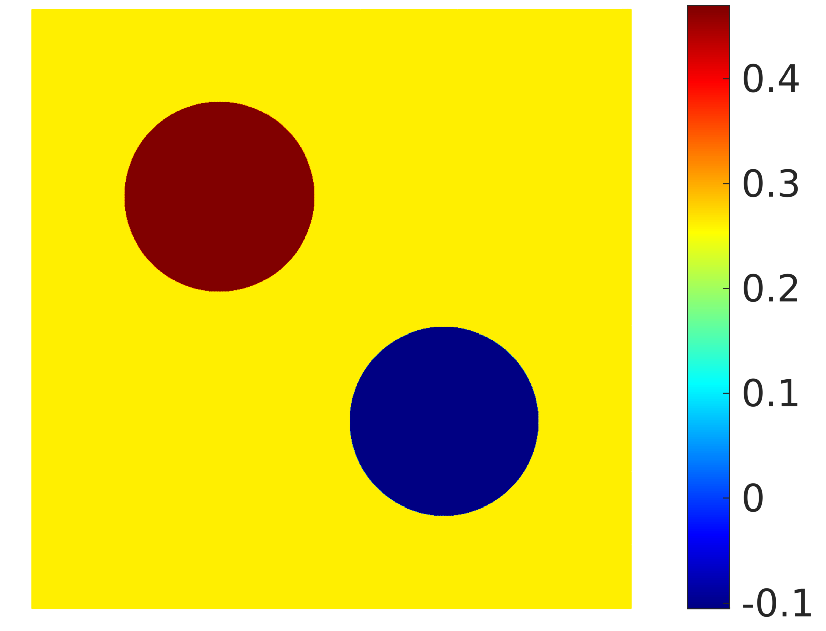
\includegraphics[width = 0.4\textwidth]{figures/sigma_exact}
\caption{Plot of the exact unknown $\sigma^*$}.
\label{fig:exact_unknown}
\end{figure}

\subsection{Results}

In Figure \ref{fig:best_solution} we plot the estimation $\sigma_{\mathrm{EnKF}}$ after $10, 50, 250$ and $500$ iterations of the ensemble Kalman algorithm. We clearly see that the approximation gets better as the number of iterations increases and that convergence has been reached, indeed we do not note a significant difference between the last two plots. We point out that we obtain a quite good approximation of the real unknown $\sigma^*$ , indeed we are trying to recover a non-continuous function in the whole domain given only some observations at the boundary.

\begin{figure}[t]
\centering
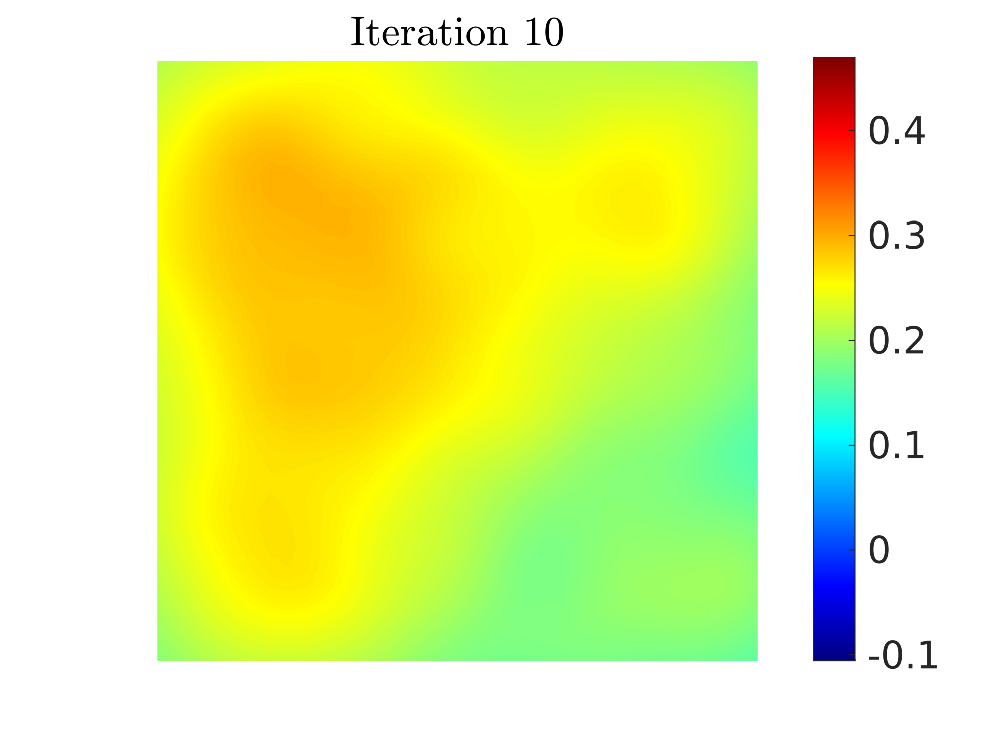
\includegraphics[width = 0.49\textwidth]{figures/ensemble_10}
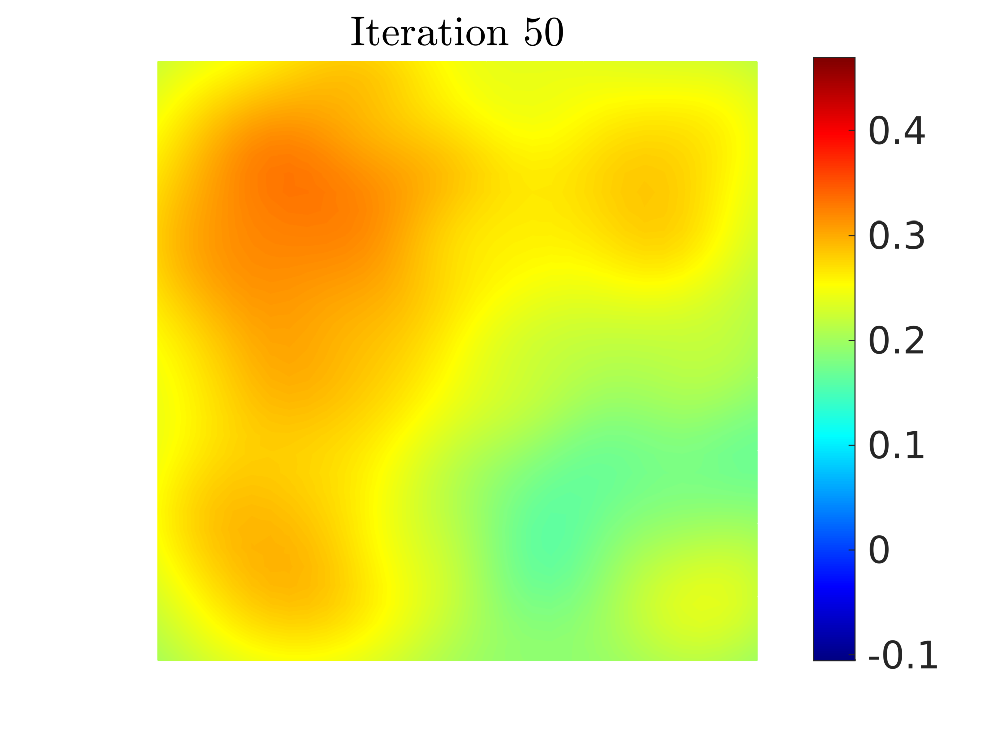
\includegraphics[width = 0.49\textwidth]{figures/ensemble_50}
\\
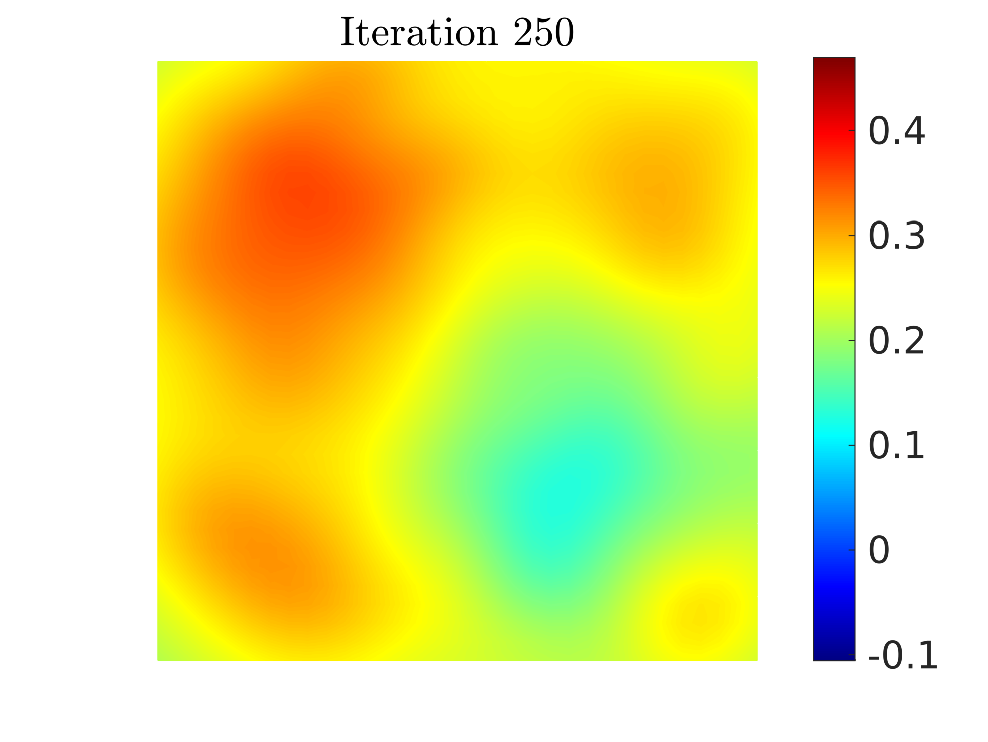
\includegraphics[width = 0.49\textwidth]{figures/ensemble_250}
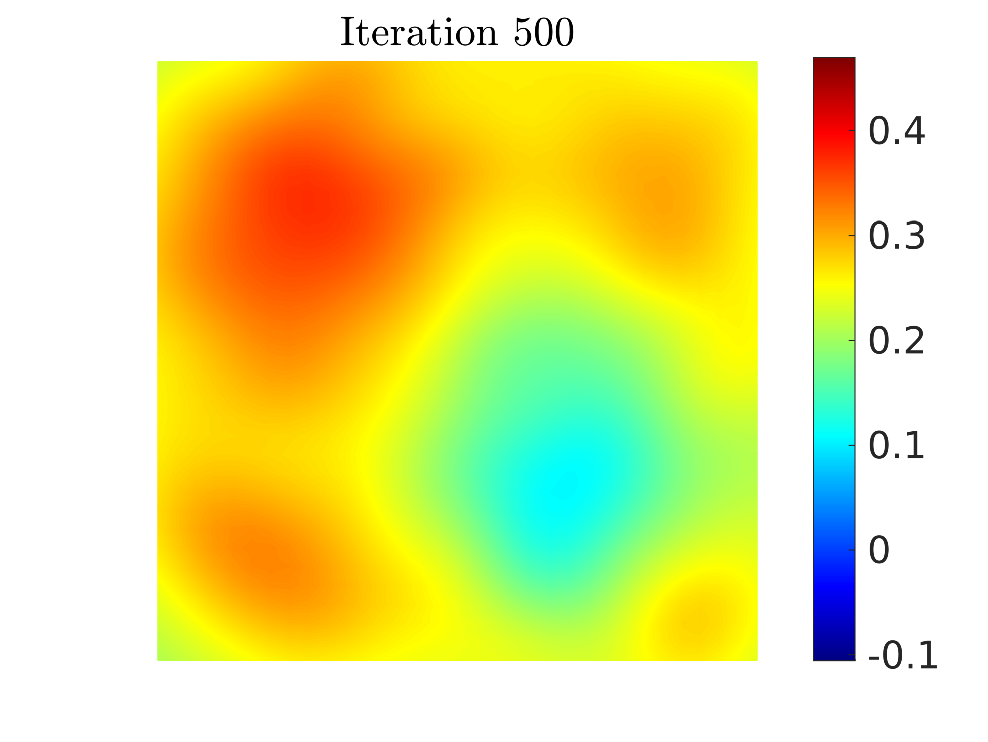
\includegraphics[width = 0.49\textwidth]{figures/ensemble_500}
\caption{Plot of the unknown $\sigma_{\mathrm{EnKF}}$ estimated by the iterative ensemble Kalman method after $10, 50, 250$ and $500$ iterations.}
\label{fig:best_solution}
\end{figure}

We perform a sensitivity analysis with respect to the dimension of the ensemble and the multiscale parameter $\varepsilon$. In Figure \ref{fig:comparison_J} we vary the number of particles $J$ and we compare the results obtained at the end of the algorithm after $500$ iterations. As expected, the approximation becomes better when the ensemble contains more particles. In particular, note that if the number of particles is too small, e.g. $J = 10$, then the approximation is completely different from the true unknown.

\begin{figure}[t]
\centering
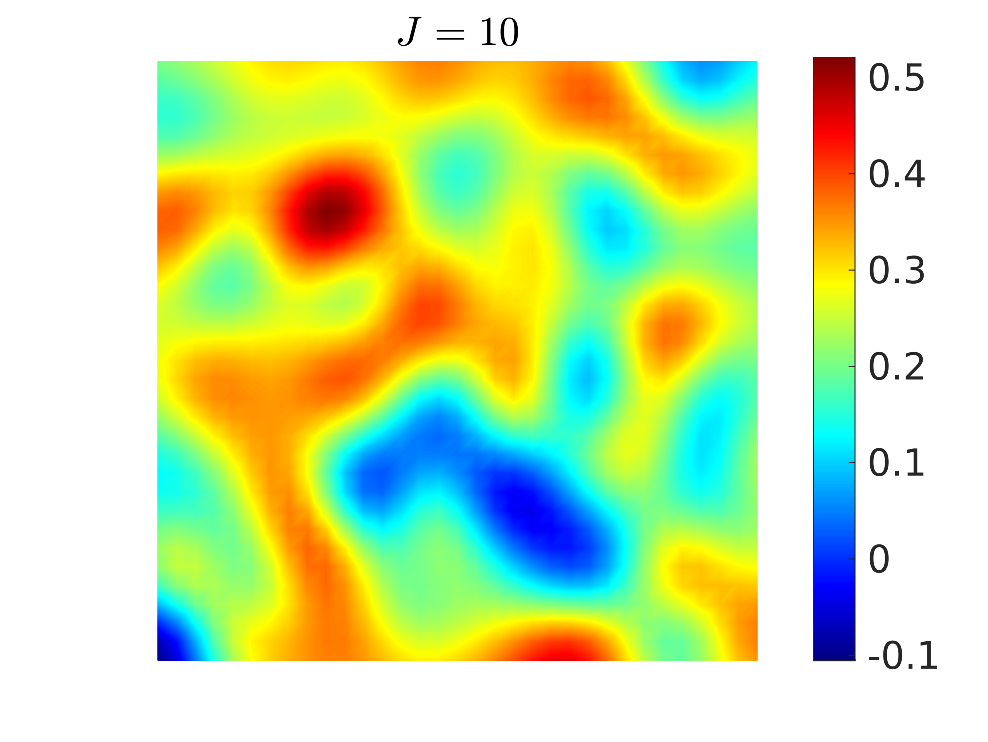
\includegraphics[width = 0.49\textwidth]{figures/ensemble_500_J10}
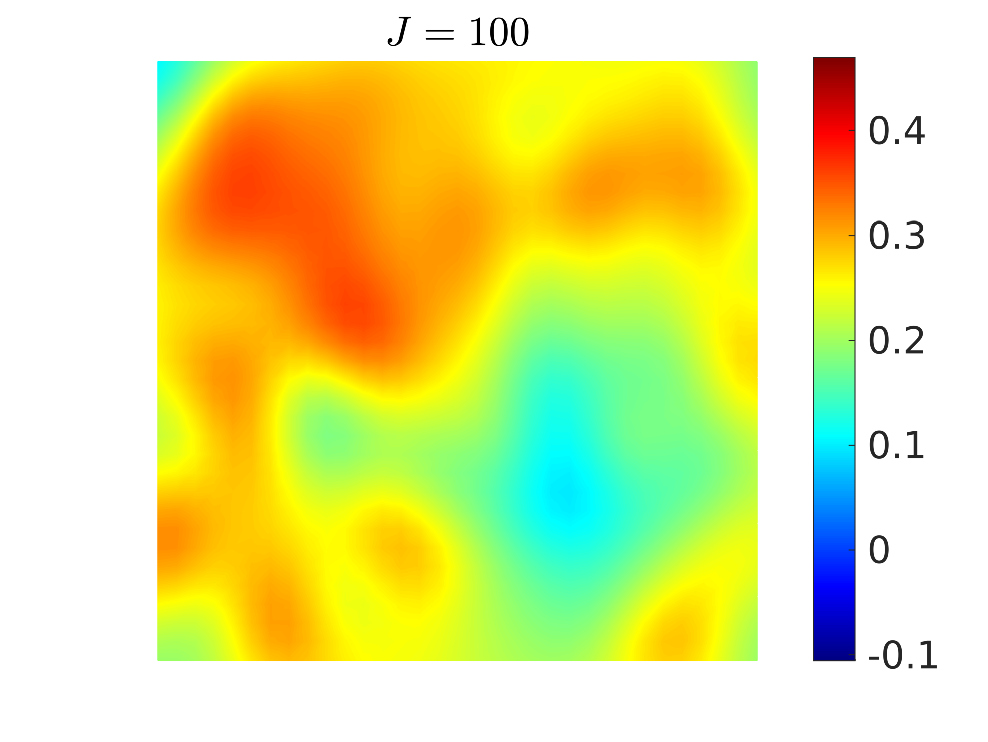
\includegraphics[width = 0.49\textwidth]{figures/ensemble_500_J100}
\\
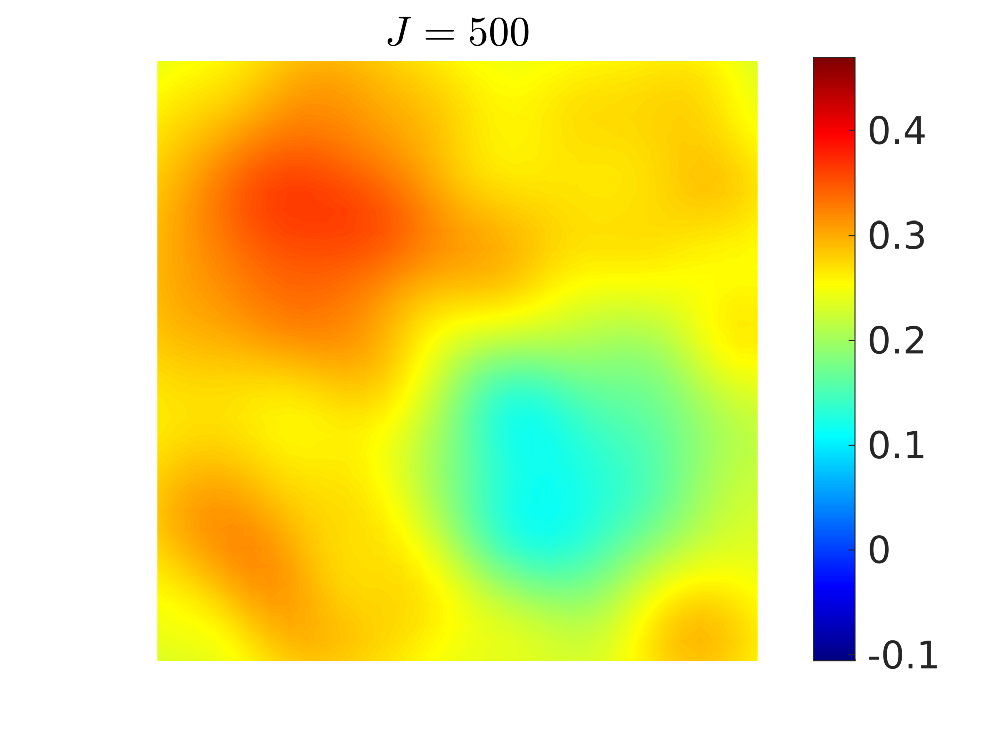
\includegraphics[width = 0.49\textwidth]{figures/ensemble_500_J500}
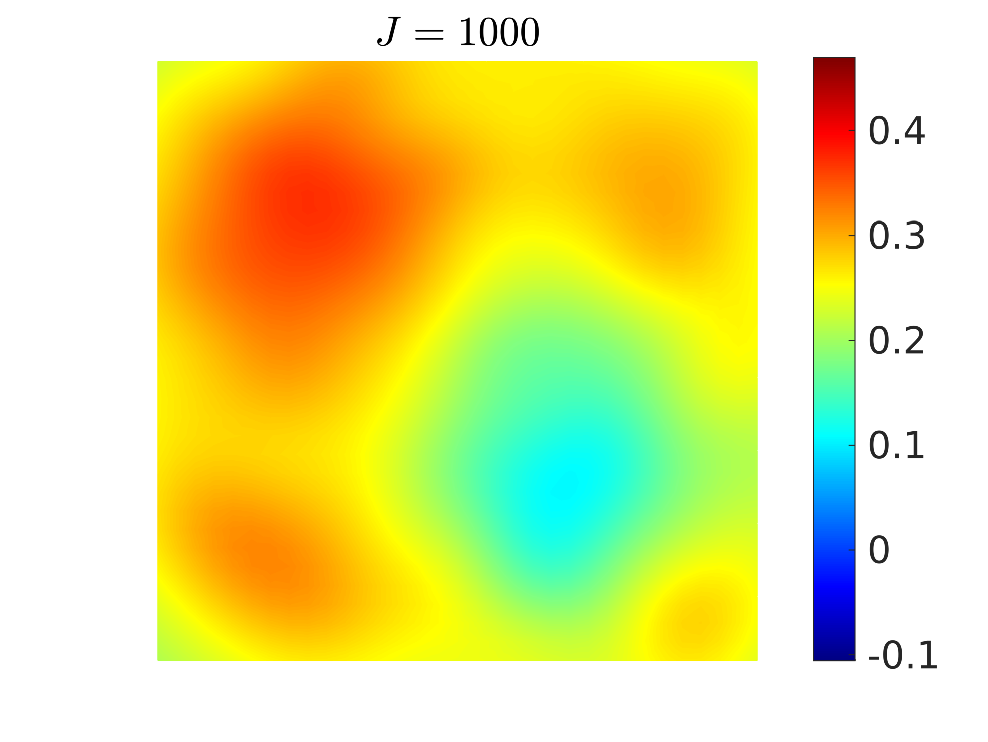
\includegraphics[width = 0.49\textwidth]{figures/ensemble_500_J1000}
\caption{Plot of the unknown $\sigma_{\mathrm{EnKF}}$ estimated by the iterative ensemble Kalman method after $500$ iterations for different numbers of particles per ensemble $J = 10, 100, 500, 1000$.}
\label{fig:comparison_J}
\end{figure}

In Figure \ref{fig:comparison_e} we compare the results obtained for different values of the multiscale parameter $\varepsilon$, in particular we take $\varepsilon = 1/4, 1/8, 1/32, 1/64$. We notice that the approximation becomes worse when $\varepsilon$ is bigger, indeed the homogenized problem becomes too different with respect to the multiscale one and, if $\varepsilon$ is too big, the solution does not approximate the true unknown.

\begin{figure}[t]
\centering
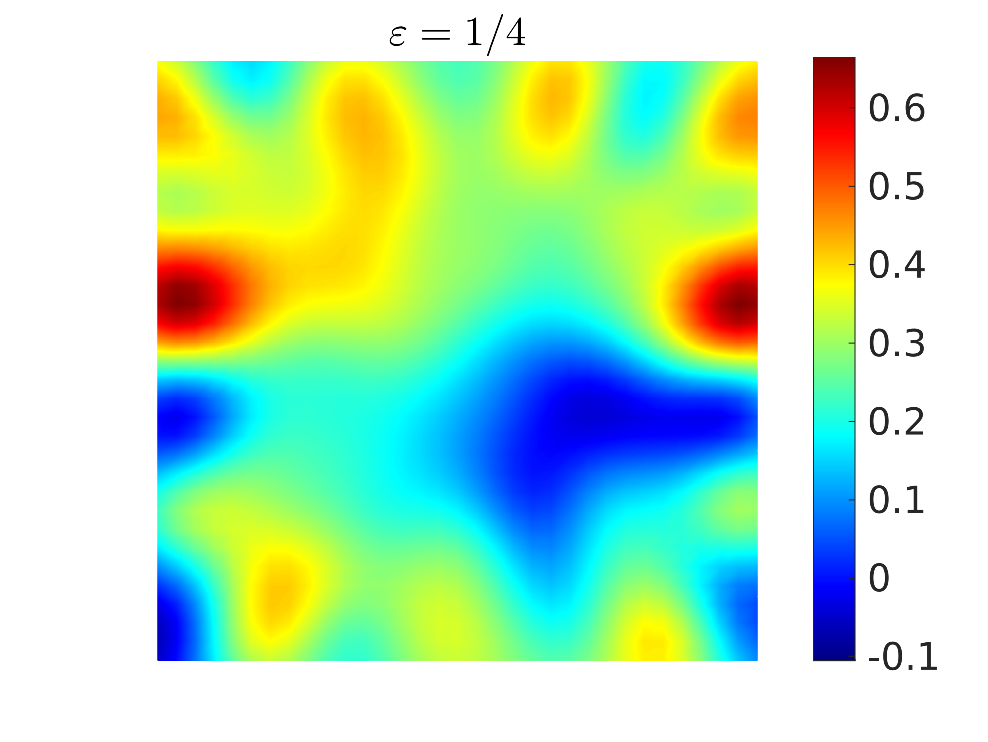
\includegraphics[width = 0.49\textwidth]{figures/ensemble_500_e4}
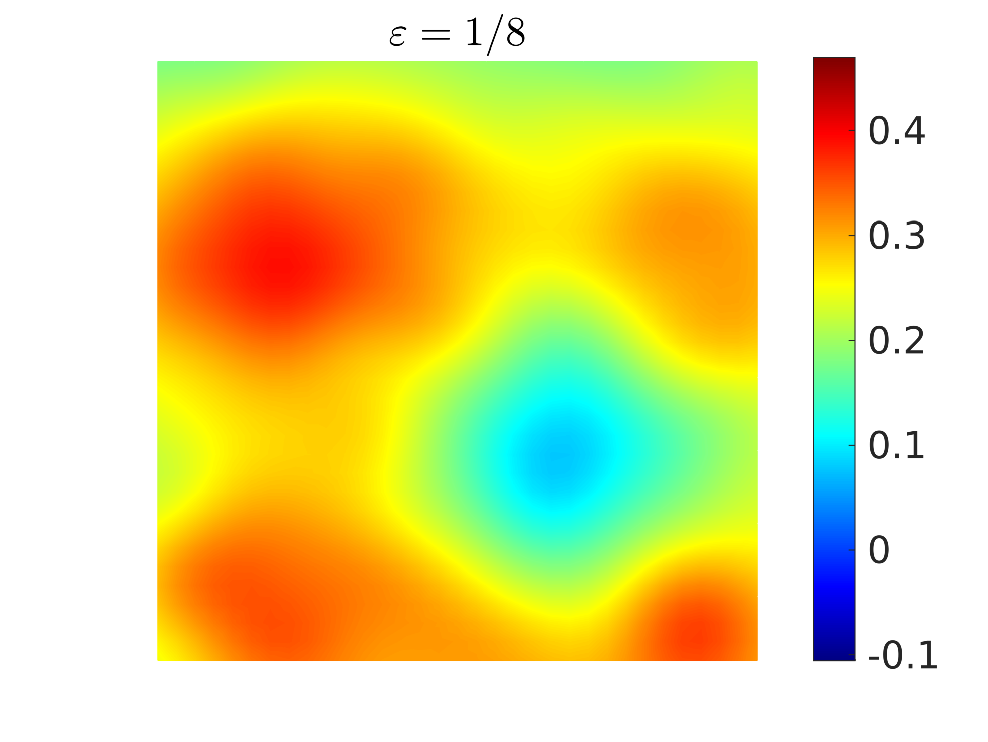
\includegraphics[width = 0.49\textwidth]{figures/ensemble_500_e8}
\\
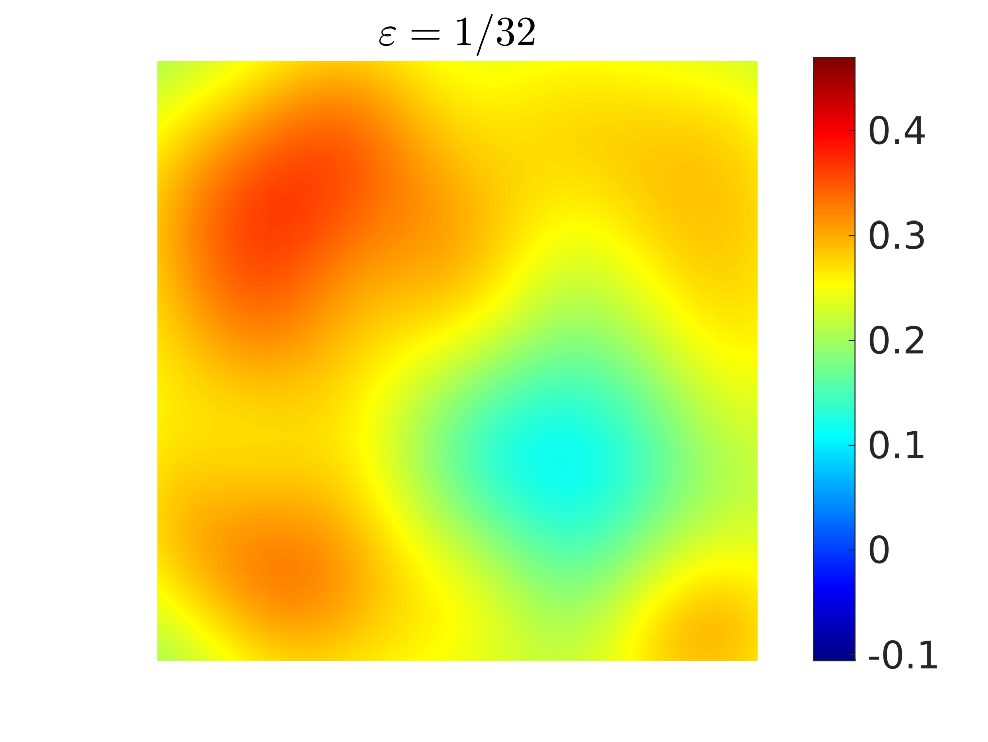
\includegraphics[width = 0.49\textwidth]{figures/ensemble_500_e32}
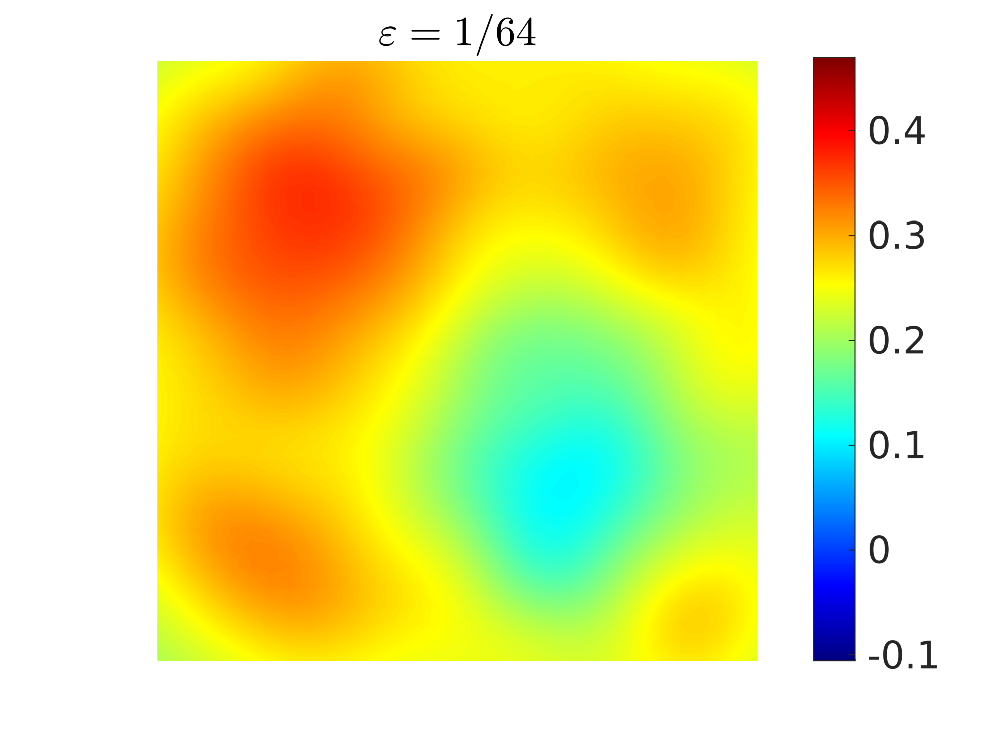
\includegraphics[width = 0.49\textwidth]{figures/ensemble_500_e64}
\caption{Plot of the unknown $\sigma_{\mathrm{EnKF}}$ estimated by the iterative ensemble Kalman method after $500$ iterations for different values of the multiscale parameter $\varepsilon = 1/4, 1/8, 1/32, 1/64$.}
\label{fig:comparison_e}
\end{figure}

Moreover, in order to obtain good results even in case $\varepsilon$ is not close to the asymptotic limit $\varepsilon \to 0$, in Figure \ref{fig:comparison_e_model_error} we apply offline modelling error estimation with $N_{\mathcal{E}} = 20$ and we plot the solution of the inverse problem \eqref{model_error_y4} for different values of the multiscale parameter $\varepsilon$. Comparing these plots with the ones in Figure \ref{fig:comparison_e}, in particular for $\varepsilon = 1/4$, we observe that the modelling error estimation significantly improves the results.

\begin{figure}[t]
\centering
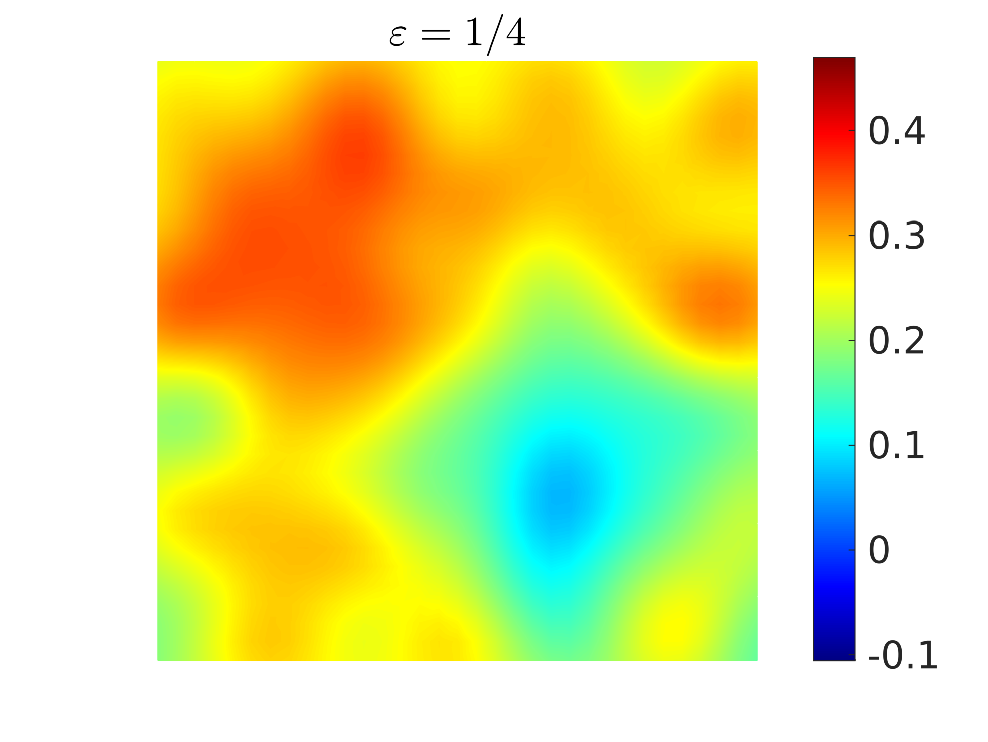
\includegraphics[width = 0.49\textwidth]{figures/ensemble_500_e4_model_error}
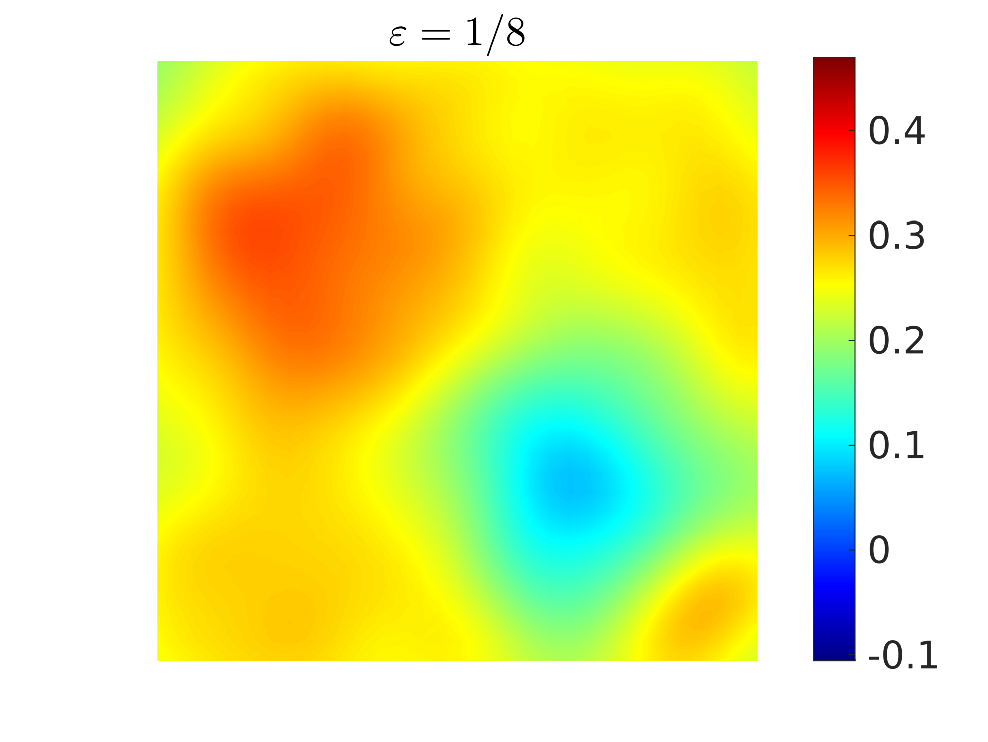
\includegraphics[width = 0.49\textwidth]{figures/ensemble_500_e8_model_error}
\\
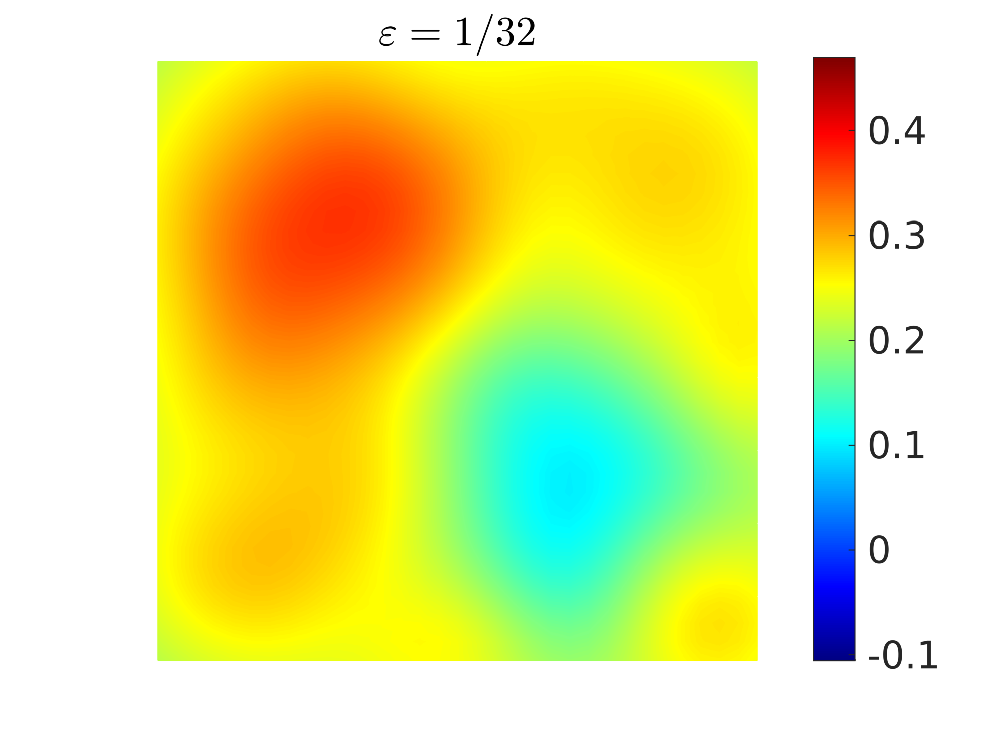
\includegraphics[width = 0.49\textwidth]{figures/ensemble_500_e32_model_error}
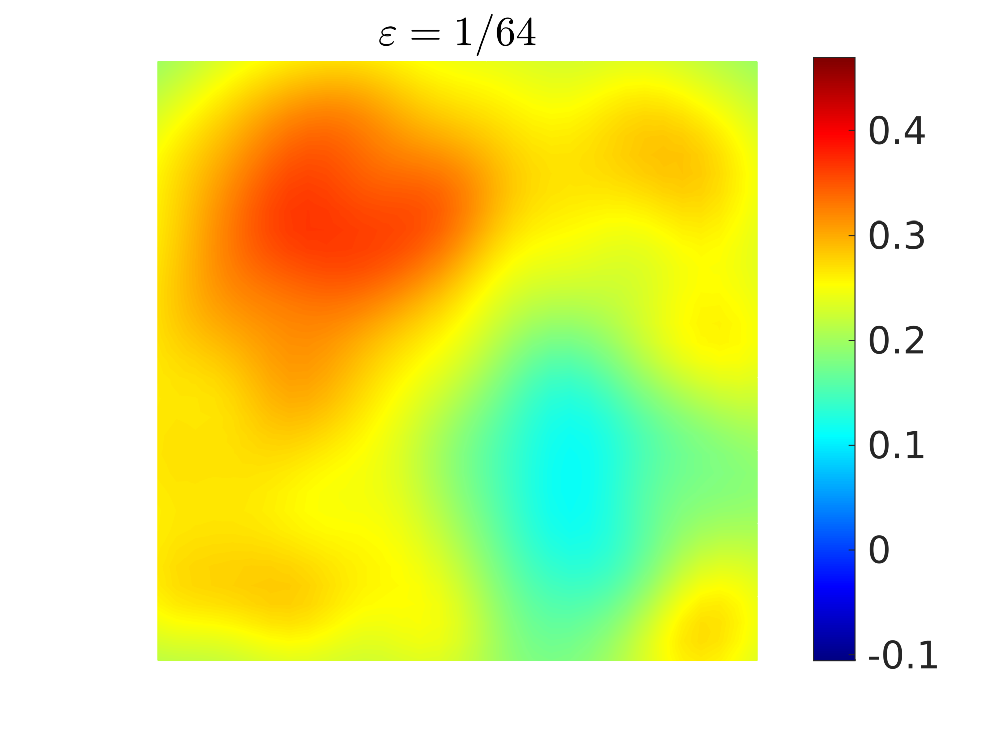
\includegraphics[width = 0.49\textwidth]{figures/ensemble_500_e64_model_error}
\caption{Plot of the unknown $\sigma_{\mathrm{EnKF}}$ estimated by the iterative ensemble Kalman method with model error estimation after $500$ iterations for different values of the multiscale parameter $\varepsilon = 1/4, 1/8, 1/32, 1/64$.}
\label{fig:comparison_e_model_error}
\end{figure}

Finally, in Figure \ref{fig:comparison_e_model_error_levels} we show the results obtained by applying the ensemble Kalman method with dynamic updating of the modelling error distribution with $\mathcal{L} = 5$ levels, $N_{\mathcal{E}}^{\ell} = 4$ samples and $N^{\ell} = 100$ iterations at each level $\ell = 1, \dots, \mathcal{L}$. The number of resolutions of the full multiscale problem is $20$ and the total number of iterations is $500$, which are equal to the previous approach, where the distribution of the modelling error was approximated offline. Comparing these plots with the ones in Figure \ref{fig:comparison_e_model_error}, we note that updating the distribution of the modelling error dynamically still improves the results.

\begin{figure}[t]
\centering
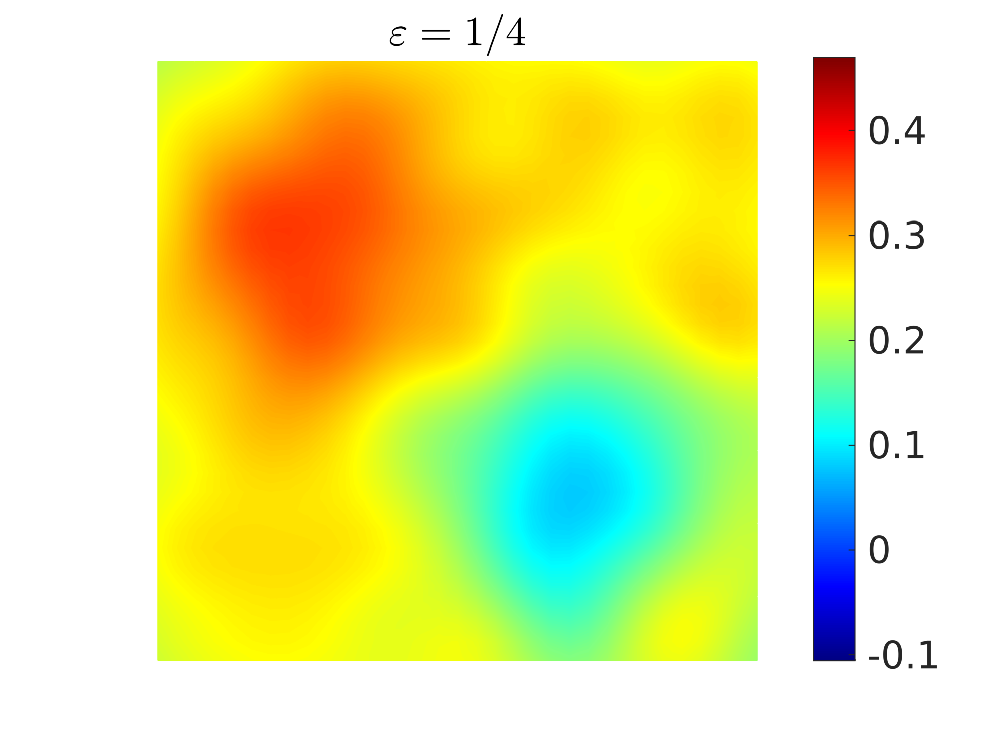
\includegraphics[width = 0.49\textwidth]{figures/ensemble_500_e4_model_error_Levels}
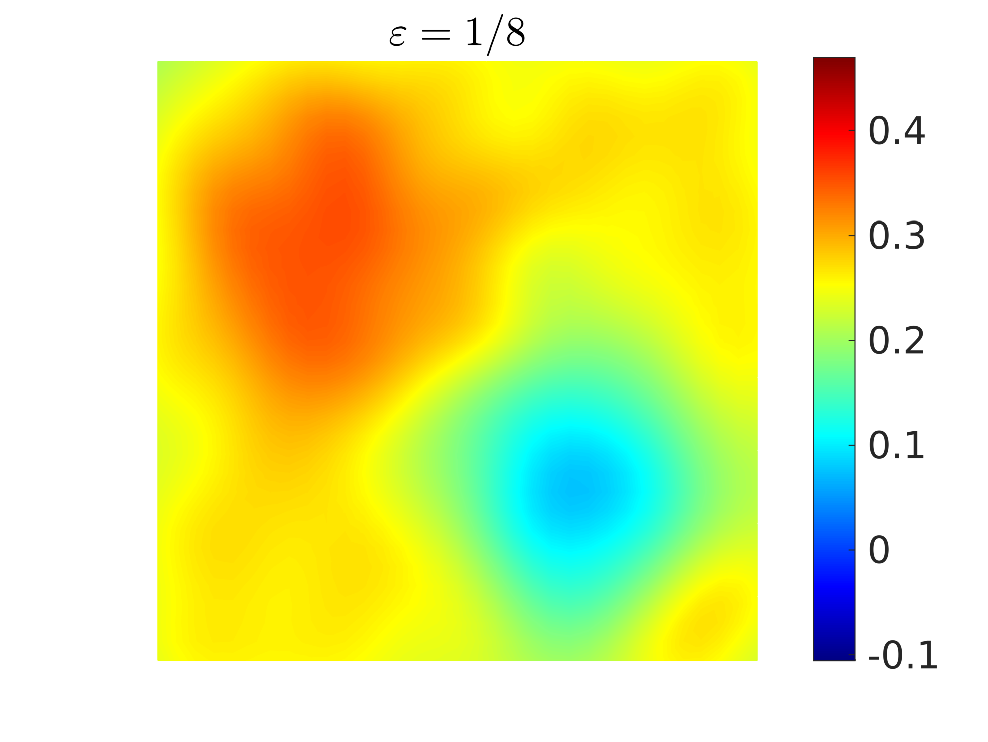
\includegraphics[width = 0.49\textwidth]{figures/ensemble_500_e8_model_error_Levels}
\\
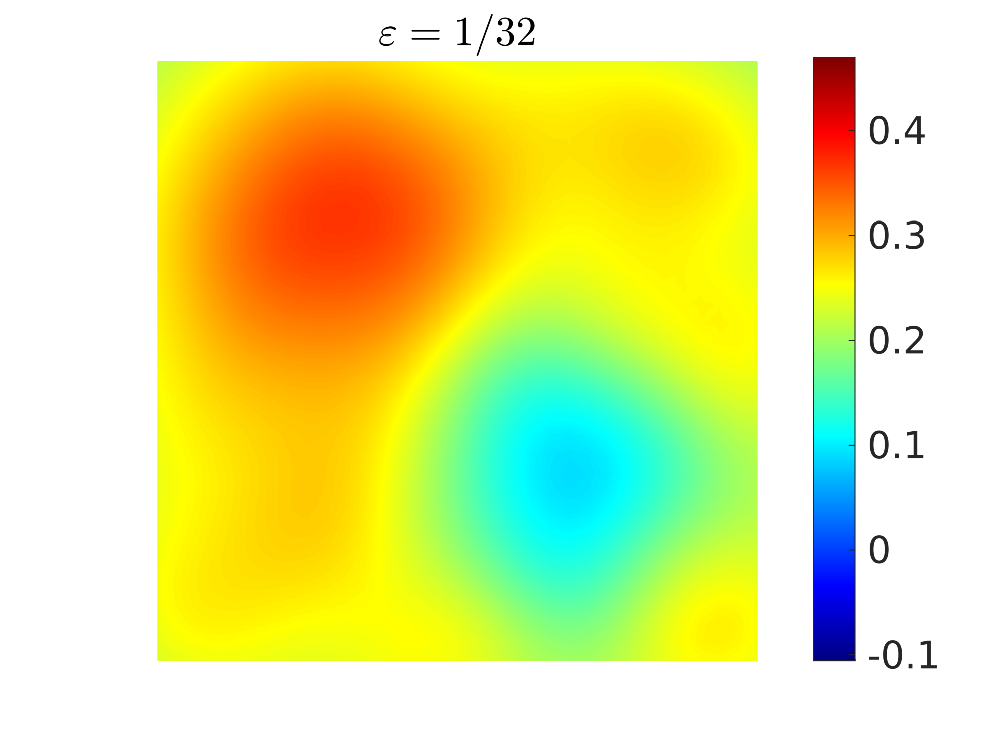
\includegraphics[width = 0.49\textwidth]{figures/ensemble_500_e32_model_error_Levels}
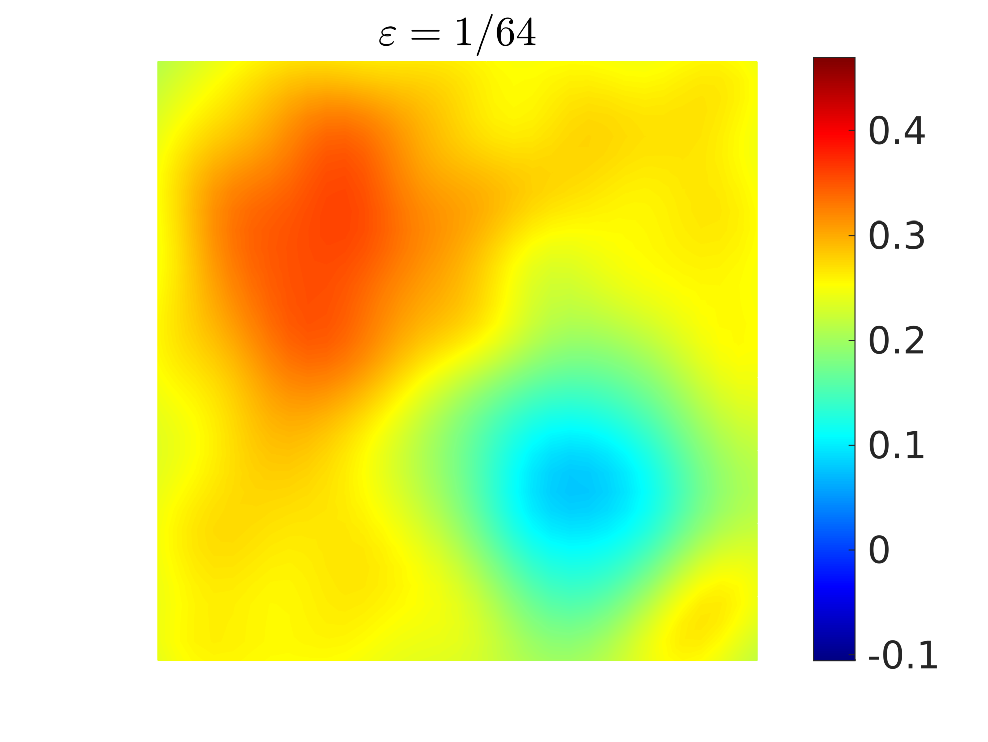
\includegraphics[width = 0.49\textwidth]{figures/ensemble_500_e64_model_error_Levels}
\caption{Plot of the unknown $\sigma_{\mathrm{EnKF}}$ estimated by the iterative ensemble Kalman method with dynamic updating of the model error estimation after $500$ iterations for different values of the multiscale parameter $\varepsilon = 1/4, 1/8, 1/32, 1/64$.}
\label{fig:comparison_e_model_error_levels}
\end{figure}

\section*{Conclusion}



\clearpage

\section*{Appendix}

\subsection*{Proof of Lemma \ref{lemma_difference_inverse}}

Note that
\[ A^{-1} - B^{-1} = A^{-1} (I - A B^{-1}) = A^{-1} (B - A) B^{-1}, \]
therefore we have
\[ \norm{A^{-1} - B^{-1}}_2 \le \norm{A^{-1}}_2 \norm{B - A}_2 \norm{B^{-1}}_2, \]
which is the desired result.

\qed

\subsection*{Proof of Lemma \ref{lemma_inverse_sum}}

Let $n$ be the dimension of the matrices, since $A$ is symmetric positive semidefinite and $B$ is symmetric positive definite, then $A + B$ is symmetric positive definite, and the eigenvalues of $A + B$ and $B$ are real and positive, thus they can be written
\[ 0 < \lambda_1(\cdot) \le \lambda_2(\cdot) \le \dots \le \lambda_n(\cdot), \]
counted with their multiplicity.
First, notice that, using the Rayleigh quotient and the fact that $x^T A x \ge 0$ for all $x$, we have
\[ \lambda_1(A + B) = \min_{x \neq 0} \frac{x^T(A + B)x}{x^T x} = \min_{x \neq 0} \frac{x^T A x + x^T B x}{x^T x} \ge \min_{x \neq 0} \frac{x^T B x}{x^T x} = \lambda_1(B), \]
which implies
\[ \norm{(A + B)^{-1}}_2 = \frac{1}{\lambda_1(A + B)} \le \frac{1}{\lambda_1(B)} = \norm{B^{-1}}_2, \]
which is the desired result.

\qed

\subsection*{Proof of Lemma \ref{G_lipschitz}}

Let $u_1, u_2 \in \mathbb{R}^M$, \corr{and $p_1 = \mathcal S(u_1)$, $p_2 = \mathcal S(u_2)$ Then, writing the weak formulations of \eqref{problem_lemma} we get
	\begin{equation*}
	\int_\Omega \big(A(u_1)\nabla p_1 - A(u_2) \nabla p_2\big) \cdot \nabla v = 0,	
	\end{equation*}
	for all $v \in H^1_0(\Omega)$. Adding and subtracting $A(u_1) \nabla p_2$ to the first factor inside the integral and rearranging terms yields}
\begin{equation*}
\int_{\Omega} A(u_1) (\nabla p_1 - \nabla p_2) \cdot \nabla v = - \int_{\Omega} (A(u_1) - A(u_2)) \nabla p_2 \cdot \nabla v.
\end{equation*}
\corr{Choosing $v = p_1 - p_2$,} using the hypotheses on $A$ and the H\"older inequality, we obtain
\begin{align*}
\alpha \norm{\nabla p_1 - \nabla p_2}_{L^2(\Omega; \R^d)}^2 \le & \;  \int_{\Omega} \left | (A(u_1) - A(u_2)) \nabla p_2 \cdot (\nabla p_1 - \nabla p_2) \right | \\
\le & \; \norm{A(u_1) - A(u_2)}_{L^{\infty}(\Omega; \R^{d \times d})} \norm{\nabla p_2}_{L^2(\Omega; \R^d)} \norm{\nabla p_1 - \nabla p_2}_{L^2(\Omega; \R^d)} \\
\le & \; M \norm{u_1 - u_2}_2 \norm{\nabla p_2}_{L^2(\Omega; \R^d)} \norm{\nabla p_1 - \nabla p_2}_{L^2(\Omega; \R^d)},
\end{align*}
which implies 
\begin{equation} \label{intermediate}
\norm{\nabla p_1 - \nabla p_2}_{L^2(\Omega; \R^d)} \le \frac{M}{\alpha} \norm{\nabla p_2}_{L^2(\Omega; \R^d)} \norm{u_1 - u_2}_2.
\end{equation}
\corr{It remains} to bound $\norm{\nabla p_2}_{L^2(\Omega; \R^N)}$, \corr{which can be achieved with a standard coercivity argument. In particular, we have
	\begin{equation} 
	\norm{\nabla p_2}_{L^2(\Omega; \R^N)} \le \frac{C_p}{\alpha} \norm{f}_{L^2(\Omega)}, 
	\end{equation}
	where $C_p$ is the Poincaré constant associated to the domain $\Omega$. Replacing in \eqref{intermediate}}, we obtain
\begin{equation*}
\norm{\nabla p_1 - \nabla p_2}_{L^2(\Omega; \R^N)} \le \frac{M C_p}{\alpha^2} \norm{f}_{L^2(\Omega)} \norm{u_1 - u_2}_2 = L_{\mathcal{S}} \norm{u_1 - u_2}_2,
\end{equation*}
which shows that $\mathcal{S}$ is Lipschitz with constant
\[ L_{\mathcal{S}} = \frac{M C_p}{\alpha^2} \norm{f}_{L^2(\Omega)}. \]
Finally, $\mathcal{G}$ is the composition of two Lipschitz operators, so it is Lipschitz \corr{of constant $L_{\mathcal G} = L_{\mathcal O} L_{\mathcal S}$}, which concludes the proof.
\qed

%\subsection*{Proof of Lemma \ref{wH1_sL2}}
%
%The sequence $\{ p^{\varepsilon} \}$ is weakly convergent in $H^1_0(\Omega)$, hence it is bounded in $H^1_0(\Omega)$. By Rellich theorem, $H^1_0(\Omega)$ is compactly embedded in $L^2(\Omega)$, so there exists a subsequence $\{ p^{\varepsilon'} \}$ such that
%\[ p^{\varepsilon'} \to \bar{p} \qquad \text{in } L^2(\Omega) \]
%for some $\bar{p}$ in $L^2(\Omega)$. Strong convergence implies weak convergence, therefore we obtain 
%\begin{equation}
%\label{convergence_pbar}
%p^{\varepsilon'} \toweak \bar{p} \qquad \text{in } L^2(\Omega).
%\end{equation}
%Moreover, since $p^{\varepsilon} \toweak p^0$ in $H^1_0(\Omega)$, we also have that this is true for the subsequence $p^{\varepsilon'}$
%\[ p^{\varepsilon'} \toweak p^0 \qquad \text{in } H^1_0(\Omega), \]
%which implies
%\begin{equation}
%\label{convergence_p0}
%p^{\varepsilon'} \toweak p^0 \qquad \text{in } L^2(\Omega).
%\end{equation}
%Thanks to (\ref{convergence_pbar}) and (\ref{convergence_p0}) and by uniqueness of the weak limit we deduce that $\bar{p} = p^0$, thus
%\[ p^{\varepsilon'} \to p^0 \qquad \text{in } L^2(\Omega). \]
%Finally, repeating this argument for subsequences, we deduce that every subsequence admits a sub-subsequence strongly converging to the same limit in $L^2(\Omega)$, hence the whole sequence strongly
%converges to $p^0$, that is
%\[ p^{\varepsilon} \to p^0 \qquad \text{in } L^2(\Omega), \]
%which is the desired result.
%
%\qed

\subsection*{Proof of Lemma \ref{f_goes_to_0}}

Let us consider an ensemble $u \in \mathcal U_{J,M}$ with particles $u^{(j)} \in \R^M$, for $j = 1, \ldots, J$. For each particle we have
\begin{align}
\norm{\mathcal{G}^{\varepsilon}(u^{(j)}) - \mathcal{G}^0(u^{(j)})}_2 = & \; \norm{\mathcal{O}(\mathcal{S}^{\varepsilon}(u^{(j)})) - \mathcal{O}(\mathcal{S}^0(u^{(j)}))}_2 \\
= & \; \norm{\mathcal{O}(p^{\varepsilon}(u^{(j)})) - \mathcal{O}(p^0(u^{(j)}))}_2 \\
\le & \; m \norm{p^{\varepsilon}(u^{(j)}) - p^0(u^{(j)})}_{L^2(\Omega)},
\end{align}
where we write explicitly the dependence of $p^{\varepsilon}$ and $p^0$ on the particle it is generated by.
By homogenization theory, we know that $p^{\varepsilon}(u^{(j)}) \toweak p^0(u^{(j)})$ in $H^1_0(\Omega)$, and therefore we have $p^{\varepsilon}(u^{(j)}) \to p^0(u^{(j)})$ in $L^2(\Omega)$, which implies
\[ e(\varepsilon, u) = \frac{1}{J} \sum_{j=1}^J \norm{\mathcal{G}^{\varepsilon}(u^{(j)}) - \mathcal{G}^0(u^{(j)})}_2 \to 0. \]
Moreover, if the solution of the homogenized problem $p^0$ is sufficiently smooth independently of $u$, namely $p^0 \in H^2(\Omega)$, letting $C > 0$ be a constant, we have for all $j = 1, \dots, J$ the following estimate, which can be found in \cite{Gri05}
\[ \norm{p^{\varepsilon}(u^{(j)}) - p^0(u^{(j)})}_{L^2(\Omega)} \le C \varepsilon, \]
hence we finally obtain
\[ e(\varepsilon, u) = \frac{1}{J} \sum_{j=1}^J \norm{\mathcal{G}^{\varepsilon}(u^{(j)}) - \mathcal{G}^0(u^{(j)})}_2 \le m C \varepsilon, \]
which proves the result for $K = m C$.

\qed

\subsection*{Proof of Lemma \ref{covariance_bound}}

Let $L$ be the Lipschitz constant of $\mathcal{G}$. For all $x \in B_R(u^*)$ we have
\begin{align*}
& \norm{\mathcal{G}(x)}_2 \le \norm{\mathcal{G}(x) - \mathcal{G}(u^*)}_2 + \norm{\mathcal{G}(u^*)}_2 \le L \norm{x - u^*}_2 + \norm{\mathcal{G}(u^*)}_2 \le LR + G, \\
& \norm{x}_2 \le \norm{x - u^*}_2 + \norm{u^*}_2 \le R + g,
\end{align*}
and we define the bounds $M = LR + G$ and $m = R + g$. The same bounds can be deduced for the mean values
\begin{align}
\label{bound_mean_u}
& \norm{\bar{u}}_2 \le \frac{1}{J} \sum_{j=1}^J \norm{u^{(j)}}_2 \le \frac{1}{J} J m = m, \\
\label{bound_mean_G}
& \norm{\bar{\mathcal{G}}}_2 \le \frac{1}{J} \sum_{j=1}^J \norm{\mathcal{G}(u^{(j)})}_2 \le \frac{1}{J} J M = M.
\end{align}
By definition of $2$-norm of a matrix we have
\begin{align*}
\norm{C^{up}(u)}_2 = & \; \sup_{x \in \mathbb{R}^L \colon \norm{x}_2 = 1} \left \lVert \frac{1}{J} \sum_{j=1}^J (u^{(j)} - \bar{u}) (\mathcal{G}(u^{(j)}) - \bar{\mathcal{G}})^T x \right \rVert_2 \\
\le & \; \sup_{x \in \mathbb{R}^L \colon \norm{x}_2 = 1} \frac{1}{J} \sum_{j=1}^J \left | (\mathcal{G}(u^{(j)}) - \bar{\mathcal{G}})^T x \right | \norm{u^{(j)} - \bar{u}}_2 \\
\le & \; \sup_{x \in \mathbb{R}^L \colon \norm{x}_2 = 1} \frac{1}{J} \sum_{j=1}^J \left \lVert \mathcal{G}(u^{(j)}) - \bar{\mathcal{G}} \right \rVert_2 \norm{x}_2 \norm{u^{(j)} - \bar{u}}_2,
\end{align*}
and using (\ref{bound_mean_u}) and (\ref{bound_mean_G}) and the fact that $\norm{x}_2 = 1$ we obtain
\begin{align*}
\norm{C^{up}(u)}_2 \le & \; \frac{1}{J} \sum_{j=1}^J \left ( \norm{\mathcal{G}(u^{(j)})}_2 + \norm{\bar{\mathcal{G}}}_2 \right ) \left ( \norm{u^{(j)}}_2 + \norm{\bar{u}}_2 \right ) \\
\le & \; \frac{1}{J} J (M + M) (m + m) = 4Mm,
\end{align*}
and we define $C_1 = 4Mm$.
The procedure is similar for the matrix $C^{pp}(u)$, where we have
\begin{align*}
\norm{C^{pp}(u)}_2 = & \; \sup_{x \in \mathbb{R}^L \colon \norm{x}_2 = 1} \left \lVert \frac{1}{J} \sum_{j=1}^J (\mathcal{G}(u^{(j)}) - \bar{\mathcal{G}}) (\mathcal{G}(u^{(j)}) - \bar{\mathcal{G}})^T x \right \rVert_2 \\
\le & \; \sup_{x \in \mathbb{R}^L \colon \norm{x}_2 = 1} \frac{1}{J} \sum_{j=1}^J \left | (\mathcal{G}(u^{(j)}) - \bar{\mathcal{G}})^T x \right | \left \lVert \mathcal{G}(u^{(j)}) - \bar{\mathcal{G}} \right \rVert_2 \\
\le & \; \sup_{x \in \mathbb{R}^L \colon \norm{x}_2 = 1} \frac{1}{J} \sum_{j=1}^J \left \lVert \mathcal{G}(u^{(j)}) - \bar{\mathcal{G}} \right \rVert^2_2 \norm{x}_2,
\end{align*}
and using bound (\ref{bound_mean_G}) and the fact that $\norm{x}_2 = 1$ we obtain
\begin{align*}
\norm{C^{up}(u)}_2 \le & \; \frac{1}{J} \sum_{j=1}^J \left ( \norm{\mathcal{G}(u^{(j)})}_2 + \norm{\bar{\mathcal{G}}}_2 \right )^2 \\
\le & \; \frac{1}{J} J (M + M)^2 = 4M^2,
\end{align*}
and we define $C_2 = 4M^2$. \\
Before proving the last two results of the lemma we need the following estimates for the ensemble of particles $u_1$ and $u_2$
\begin{align*}
\norm{\bar{u}_1 - \bar{u}_2}_2 = & \; \left \lVert \frac{1}{J} \sum_{j=1}^J (u_1^{(j)} - u_2^{(j)}) \right \rVert_2 \le \frac{1}{J} \sum_{j=1}^J \norm{u_1^{(j)} - u_2^{(j)}}_2 = \norm{u_1 - u_2}, \\
\norm{\bar{\mathcal{G}}_1 - \bar{\mathcal{G}}_2}_2 = & \; \left \lVert \frac{1}{J} \sum_{j=1}^J (\mathcal{G}(u_1^{(j)}) - \mathcal{G}(u_2^{(j)})) \right \rVert_2 \le \frac{1}{J} \sum_{j=1}^J \norm{\mathcal{G}(u_1^{(j)}) - \mathcal{G}(u_2^{(j)})}_2 \\
& \hspace{137pt} \le L \frac{1}{J} \sum_{j=1}^J \norm{u_1^{(j)} - u_2^{(j)}}_2 \\
& \hspace{137pt} = L \norm{u_1 - u_2}.
\end{align*}
By definition of $2$ norm of a matrix and using the triangle inequality we have
\begin{align*}
& \norm{C^{up}(u_1) - C^{up}(u_2)}_2 \\
& \qquad = \sup_{x \in \mathbb{R}^L \colon \norm{x}_2 = 1} \left \lVert \frac{1}{J} \sum_{j=1}^J \left [ (u_1^{(j)} - \bar{u}_1) (\mathcal{G}(u_1^{(j)}) - \bar{\mathcal{G}}_1)^T x - (u_2^{(j)} - \bar{u}_2) (\mathcal{G}(u_2^{(j)}) - \bar{\mathcal{G}}_2)^T x \right ] \right \rVert_2 \\
& \qquad \le \quad \sup_{x \in \mathbb{R}^L \colon \norm{x}_2 = 1} \frac{1}{J} \sum_{j=1}^J \left \lVert (u_1^{(j)} - \bar{u}_1) (\mathcal{G}(u_1^{(j)}) - \bar{\mathcal{G}}_1)^T x - (u_1^{(j)} - \bar{u}_1) (\mathcal{G}(u_2^{(j)}) - \bar{\mathcal{G}}_2)^T x \right \rVert_2 \\
& \qquad \quad + \sup_{x \in \mathbb{R}^L \colon \norm{x}_2 = 1} \frac{1}{J} \sum_{j=1}^J \left \lVert (u_1^{(j)} - \bar{u}_1) (\mathcal{G}(u_2^{(j)}) - \bar{\mathcal{G}}_2)^T x - (u_2^{(j)} - \bar{u}_2) (\mathcal{G}(u_2^{(j)}) - \bar{\mathcal{G}}_2)^T x \right \rVert_2,
\end{align*}
which implies
\begin{align*}
& \norm{C^{up}(u_1) - C^{up}(u_2)}_2 \\
& \qquad \le \quad \sup_{x \in \mathbb{R}^L \colon \norm{x}_2 = 1} \frac{1}{J} \sum_{j=1}^J \left \lVert (u_1^{(j)} - \bar{u}_1) [ (\mathcal{G}(u_1^{(j)}) - \mathcal{G}(u_2^{(j)})) + (\bar{\mathcal{G}}_2 - \bar{\mathcal{G}}_1)]^T x ] \right \rVert_2 \\
& \qquad \quad + \sup_{x \in \mathbb{R}^L \colon \norm{x}_2 = 1} \frac{1}{J} \sum_{j=1}^J \left \lVert [ (u_1^{(j)} - u_2^{(j)}) + (\bar{u}_2 - \bar{u}_1) ] (\mathcal{G}(u_2^{(j)}) - \bar{\mathcal{G}}_2)^T x \right \rVert_2 \\ 
& \qquad \le \quad \sup_{x \in \mathbb{R}^L \colon \norm{x}_2 = 1} \frac{1}{J} \sum_{j=1}^J \norm{u_1^{(j)} - \bar{u}_1}_2 [ \norm{\mathcal{G}(u_1^{(j)}) - \mathcal{G}(u_2^{(j)})}_2 + \norm{\bar{\mathcal{G}}_2 - \bar{\mathcal{G}}_1}_2 ] \norm{x}_2 \\
& \qquad \quad + \sup_{x \in \mathbb{R}^L \colon \norm{x}_2 = 1} \frac{1}{J} \sum_{j=1}^J [ \norm{u_1^{(j)} - u_2^{(j)}}_2 + \norm{\bar{u}_2 - \bar{u}_1}_2 ] \norm{\mathcal{G}(u_2^{(j)}) - \bar{\mathcal{G}}_2} \norm{x}_2.
\end{align*}
Using bounds (\ref{bound_mean_u}) and (\ref{bound_mean_G}) and the fact that $\mathcal{G}$ is Lipschitz with constant $L$, we obtain
\begin{align*}
& \norm{C^{up}(u_1) - C^{up}(u_2)}_2 \\
& \qquad \le \frac{1}{J} \sum_{j=1}^J \left \{ (\norm{u_1^{(j)}}_2 + \norm{\bar{u}_1}_2) (L \norm{u_1^{(j)} - u_2^{(j)}}_2 + L \norm{u_1 - u_2}) \right \} \\
& \qquad \qquad + \frac{1}{J} \sum_{j=1}^J \left \{ (\norm{u_1^{(j)} - u_2^{(j)}}_2 + \norm{\bar{u}_2 - \bar{u}_1}_2) (\norm{\mathcal{G}(u_2^{(j)})}_2 + \norm{\bar{\mathcal{G}}_2}_2) \right \} \\
& \qquad \le \frac{1}{J} \sum_{j=1}^J \left \{ 2m ( LJ \norm{u_1 - u_2} + L \norm{u_1 - u_2} ) + ( J \norm{u_1 - u_2} + \norm{u_1 - u_2} ) 2M \right \} \\
& \qquad \le 2 (J+1) \max \{ mL, M \} \norm{u_1 - u_2},
\end{align*}
and we define $C_3 = 2 (J+1) \max \{ mL, M \}$. The computation is similar for the last point of the statement, for which we have
\begin{align*}
& \norm{C^{pp}(u_1) - C^{pp}(u_2)}_2 \\
& \qquad = \sup_{x \in \mathbb{R}^L \colon \norm{x}_2 = 1} \left \lVert \frac{1}{J} \sum_{j=1}^J \left [ (\mathcal{G}(u_1^{(j)}) - \bar{\mathcal{G}}_1) (\mathcal{G}(u_1^{(j)}) - \bar{\mathcal{G}}_1)^T x - (\mathcal{G}(u_2^{(j)}) - \bar{\mathcal{G}}_2) (\mathcal{G}(u_2^{(j)}) - \bar{\mathcal{G}}_2)^T x \right ] \right \rVert_2 \\
& \qquad \le \quad \sup_{x \in \mathbb{R}^L \colon \norm{x}_2 = 1} \frac{1}{J} \sum_{j=1}^J \left \lVert (\mathcal{G}(u_1^{(j)}) - \bar{\mathcal{G}}_1) (\mathcal{G}(u_1^{(j)}) - \bar{\mathcal{G}}_1)^T x - (\mathcal{G}(u_1^{(j)}) - \bar{\mathcal{G}}_1) (\mathcal{G}(u_2^{(j)}) - \bar{\mathcal{G}}_2)^T x \right \rVert_2 \\
& \qquad \quad + \sup_{x \in \mathbb{R}^L \colon \norm{x}_2 = 1} \frac{1}{J} \sum_{j=1}^J \left \lVert (\mathcal{G}(u_1^{(j)}) - \bar{\mathcal{G}}_1) (\mathcal{G}(u_2^{(j)}) - \bar{\mathcal{G}}_2)^T x - (\mathcal{G}(u_2^{(j)}) - \bar{\mathcal{G}}_2) (\mathcal{G}(u_2^{(j)}) - \bar{\mathcal{G}}_2)^T x \right \rVert_2, 
\end{align*}
which implies
\begin{align*}
& \norm{C^{pp}(u_1) - C^{pp}(u_2)}_2 \\
& \qquad \le \quad \sup_{x \in \mathbb{R}^L \colon \norm{x}_2 = 1} \frac{1}{J} \sum_{j=1}^J \left \lVert (\mathcal{G}(u_1^{(j)}) - \bar{\mathcal{G}}_1) [ (\mathcal{G}(u_1^{(j)}) - \mathcal{G}(u_2^{(j)})) + (\bar{\mathcal{G}}_2 - \bar{\mathcal{G}}_1)]^T x ] \right \rVert_2 \\
& \qquad \quad + \sup_{x \in \mathbb{R}^L \colon \norm{x}_2 = 1} \frac{1}{J} \sum_{j=1}^J \left \lVert [ (\mathcal{G}(u_1^{(j)}) - \mathcal{G}(u_2^{(j)})) + (\bar{\mathcal{G}}_2 - \bar{\mathcal{G}}_1) ] (\mathcal{G}(u_2^{(j)}) - \bar{\mathcal{G}}_2)^T x \right \rVert_2 , \\
& \qquad \le \quad \sup_{x \in \mathbb{R}^L \colon \norm{x}_2 = 1} \frac{1}{J} \sum_{j=1}^J \norm{\mathcal{G}(u_1^{(j)}) - \bar{\mathcal{G}}_1}_2 [ \norm{\mathcal{G}(u_1^{(j)}) - \mathcal{G}(u_2^{(j)})}_2 + \norm{\bar{\mathcal{G}}_2 - \bar{\mathcal{G}}_1}_2 ] \norm{x}_2 \\
& \qquad \quad + \sup_{x \in \mathbb{R}^L \colon \norm{x}_2 = 1} \frac{1}{J} \sum_{j=1}^J [ \norm{\mathcal{G}(u_1^{(j)}) - \mathcal{G}(u_2^{(j)})}_2 + \norm{\bar{\mathcal{G}}_2 - \bar{\mathcal{G}}_1}_2 ] \norm{\mathcal{G}(u_2^{(j)}) - \bar{\mathcal{G}}_2} \norm{x}_2.
\end{align*}
Using bounds (\ref{bound_mean_u}) and (\ref{bound_mean_G}) and the fact that $\mathcal{G}$ is Lipschitz with constant $L$, we obtain
\begin{align*}
& \norm{C^{pp}(u_1) - C^{pp}(u_2)}_2 \\
& \qquad \le \frac{1}{J} \sum_{j=1}^J \left \{ 2M ( LJ \norm{u_1 - u_2} + L \norm{u_1 - u_2} ) + ( LJ \norm{u_1 - u_2} + L \norm{u_1 - u_2} ) 2M \right \} \\
& \qquad = 4 M L (J+1) \norm{u_1 - u_2},
\end{align*}
and we define $C_4 = 4 M L (J+1)$.

\qed

\subsection*{Proof of Lemma \ref{fh_goes_to_0}}

\corr{Let us consider an ensemble $u \in \mathcal U_{J,M}$ with particles $u^{(j)} \in \R^M$, for $j = 1, \ldots, J$. For each particle we have 
\begin{align}
\norm{\mathcal{G}^0_h(u^{(j)}) - \mathcal{G}^0(u^{(j)})}_2 = & \; \norm{\mathcal{O}(\mathcal{S}^0_h(u^{(j)})) - \mathcal{O}(\mathcal{S}^0(u^{(j)}))}_2 \\
= & \; \norm{\mathcal{O}(p^0_h(u^{(j)})) - \mathcal{O}(p^0(u^{(j)}))}_2 \\
\le & \; m \norm{p^0_h(u^{(j)}) - p^0(u^{(j)})}_{L^2(\Omega)},
\end{align}
where we write explicitly the dependence of $p^0$ and $p^0_h$ on the particle it is generated by. We now consider the standard a priori error estimates of FEM, (see e.g. \cite[Theorem 3.2.5]{Cia02}), which reads
\[ \norm{p^0_h(u^{(j)}) - p^0(u^{(j)})}_{L^2(\Omega)} \le C \abs{p(u^{(j)})}_{H^{s+1}(\Omega)} h^{s+1}. \]
Moreover, higher order boundary regularity results for elliptic partial differential equations (see e.g. \cite[Theorem 6.3.5]{Eva10}), imply for a constant $\tilde{C} > 0$ and for all $j = 1, \ldots, J$
\[ \norm{p^0_h(u^{(j)}) - p^0(u^{(j)})}_{L^2(\Omega)} \leq \norm{f}_{H^{q-1}(\Omega)} h^{s+1}. \]
Finally, we obtain
\begin{align}
\tilde{e}(h, u) &= \; \frac1J \sum_{j=1}^J \norm{\mathcal{G}^0_h(u^{(j)}) - \mathcal{G}^0(u^{(j)})}_2\\
&\le m C \tilde{C} \norm{f}_{H^{q-1}(\Omega)} h^{s+1},
\end{align}
which proves the result for $\tilde{K} = m C \tilde{C} \norm{f}_{H^{q-1}(\Omega)}$.}
\qed

\subsection*{Proof of Lemma \ref{equivalence_convergence_DW1}}

We recall the duality formula (\ref{Wasserstein_dual}) for the Wasserstein distance $W_{1,s}$
\[ W_{1,s}(\mu_n, \mu) = \sup_{\varphi \in \Phi} \left \{ \int_{B_R(u^*)} \varphi d(\mu_n - \mu) \right \}, \]
where $\Phi$ is the set of all globally Lipschitz continuous functions $\varphi \colon B_R(u^*) \to \R$ with Lipschitz constant $L \le 1$. Note that if $\varphi \in \Phi$, then also $- \varphi \in \Phi$.
Therefore we deduce that
\begin{equation}
\label{equality_absolute_value}
W_{1,s}(\mu_n, \mu) = \sup_{\varphi \in \Phi} \left \{ \int_{B_R(u^*)} \varphi d(\mu_n - \mu) \right \} = \sup_{\varphi \in \Phi} \left \{ \left | \int_{B_R(u^*)} \varphi d(\mu_n - \mu) \right | \right \}.
\end{equation}
Indeed we have
\[ \int_{B_R(u^*)} \varphi d(\mu_n - \mu) \le \left | \int_{B_R(u^*)} \varphi d(\mu_n - \mu) \right |, \]
which implies the first inequality
\[ \sup_{\varphi \in \Phi} \left \{ \int_{B_R(u^*)} \varphi d(\mu_n - \mu) \right \} \le \sup_{\varphi \in \Phi} \left \{ \left | \int_{B_R(u^*)} \varphi d(\mu_n - \mu) \right | \right \}. \]
On the other hand, we also have
\begin{equation}
\label{inequality_sets}
A = \left \{ \int_{B_R(u^*)} \varphi d(\mu_n - \mu) \colon \varphi \in \Phi \right \} \supseteq \left \{ \left | \int_{B_R(u^*)} \varphi d(\mu_n - \mu) \right | \colon \varphi \in \Phi \right \} = A',
\end{equation}
because if $c \in A'$, which means that there exists $\varphi \in \Phi$ such that
\[ c = \left | \int_{B_R(u^*)} \varphi d(\mu_n - \mu) \right |, \]
then we can take $\tilde{\varphi} \in \Phi$ defined as
\begin{equation*}
\tilde{\varphi} = 
\begin{cases}
\varphi & \text{ if } \int_{B_R(u^*)} \varphi d(\mu_n - \mu) > 0 \\
- \varphi & \text{ if } \int_{B_R(u^*)} \varphi d(\mu_n - \mu) < 0, \\
\end{cases}
\end{equation*}
and note that that 
\[ c = \int_{B_R(u^*)} \tilde{\varphi} d(\mu_n - \mu), \]
which implies that $c \in A$. Therefore, by (\ref{inequality_sets}), we deduce the opposite inequality
\[ \sup_{\varphi \in \Phi} \left \{ \int_{B_R(u^*)} \varphi d(\mu_n - \mu) \right \} \ge \sup_{\varphi \in \Phi} \left \{ \left | \int_{B_R(u^*)} \varphi d(\mu_n - \mu) \right | \right \}. \]
Then, thanks to (\ref{equality_absolute_value}), we have
\begin{align*}
\sup_{\varphi \in \Phi} \mathbb{E}_{\xi} \left [ \left | \int_{B_R(u^*)} \varphi d(\mu_n - \mu) \right | \right ] \le & \; \mathbb{E}_{\xi} \left [ \sup_{\varphi \in \Phi} \left \{ \left | \int_{B_R(u^*)} \varphi d(\mu_n - \mu) \right | \right \} \right ] \\
= & \; \mathbb{E}_{\xi} [ W_{1,s}(\mu_n, \mu) ],
\end{align*}
and the right hand side vanishes by hypothesis, so we obtain
\[ \sup_{\varphi \in \Phi} \mathbb{E}_{\xi} \left [ \left | \int_{B_R(u^*)} \varphi d(\mu_n - \mu) \right | \right ] \to 0. \]
Hence
\begin{equation}
\label{for_all_phi}
\mathbb{E}_{\xi} \left [ \left | \int_{B_R(u^*)} \varphi d \mu_n - \int_{B_R(u^*)} \varphi d \mu \right | \right ] \to 0 \qquad \text{for all } \varphi \in \Phi.
\end{equation}
It remains to show that (\ref{for_all_phi}) holds true for all functions $f \in C^0(B_R(u^*))$. First, we consider any Lipschitz function $\psi$ with Lipschitz constant $L$. We define $\phi = \psi/L$, then $\phi \in \Phi$, indeed
\begin{equation*}
\abs{\phi(x) - \phi(y)} = \left | \frac{1}{L} \psi(x) - \frac{1}{L} \psi(y) \right | = \frac{1}{L} \abs{\psi(x) - \psi(y)} \le \frac{1}{L} L \norm{x - y}_s = \norm{x - y}_s.
\end{equation*}
Therefore we have
\begin{equation}
\label{for_all_psi}
\mathbb{E}_{\xi} \left [ \left | \int_{B_R(u^*)} \psi d \mu_n - \int_{B_R(u^*)} \psi d \mu \right | \right ] = L \mathbb{E}_{\xi} \left [ \left | \int_{B_R(u^*)} \phi d \mu_n - \int_{B_R(u^*)} \phi d \mu \right | \right ] \to 0.
\end{equation}
By density, any continuous bounded function $f \in C^0(B_R(u^*))$ can be approximated by a sequence of Lipschitz functions $\{ \psi_k \}_{k \in \mathbb{N}}$ such that $\norm{\psi_k}_{L^{\infty}(B_R(u^*))} \le C$ for all $k \in \mathbb{N}$ where $C$ is a constant dependent on $f$ and $\norm{\psi_k - f}_{L^{\infty}(B_R(u^*))} \to 0$ as $k \to \infty$. Thanks to (\ref{for_all_psi}) we have
\[ \mathbb{E}_{\xi} \left [ \left | \int_{B_R(u^*)} \psi_k d \mu_n - \int_{B_R(u^*)} \psi_k d \mu \right | \right ] \to 0, \]
and, applying Lebesgue dominated convergence theorem, we can pass to the limit as $k \to \infty$. We can exchange the limit with the expectation and the integral because the integrand functions are bounded by $C$ and the measures $\mu_n$ and $\mu$ are finite, since they are probability measures. Thus we obtain
\[ \mathbb{E}_{\xi} \left [ \left | \int_{B_R(u^*)} f d \mu_n - \int_{B_R(u^*)} f d \mu \right | \right ] \to 0, \]
for all bounded continuous functions $f \in C^0(B_R(u^*))$ which means
\[ \mu_n \xrightharpoonup{L^1} \mu, \]
which is the desired result.

\qed

\bibliographystyle{siam}
\bibliography{anmc}

\end{document}